% Options for packages loaded elsewhere
\PassOptionsToPackage{unicode}{hyperref}
\PassOptionsToPackage{hyphens}{url}
%
\documentclass[
]{article}
\usepackage{amsmath,amssymb}
\usepackage{lmodern}
\usepackage{iftex}
\ifPDFTeX
  \usepackage[T1]{fontenc}
  \usepackage[utf8]{inputenc}
  \usepackage{textcomp} % provide euro and other symbols
\else % if luatex or xetex
  \usepackage{unicode-math}
  \defaultfontfeatures{Scale=MatchLowercase}
  \defaultfontfeatures[\rmfamily]{Ligatures=TeX,Scale=1}
\fi
% Use upquote if available, for straight quotes in verbatim environments
\IfFileExists{upquote.sty}{\usepackage{upquote}}{}
\IfFileExists{microtype.sty}{% use microtype if available
  \usepackage[]{microtype}
  \UseMicrotypeSet[protrusion]{basicmath} % disable protrusion for tt fonts
}{}
\makeatletter
\@ifundefined{KOMAClassName}{% if non-KOMA class
  \IfFileExists{parskip.sty}{%
    \usepackage{parskip}
  }{% else
    \setlength{\parindent}{0pt}
    \setlength{\parskip}{6pt plus 2pt minus 1pt}}
}{% if KOMA class
  \KOMAoptions{parskip=half}}
\makeatother
\usepackage{xcolor}
\usepackage[margin=1in]{geometry}
\usepackage{color}
\usepackage{fancyvrb}
\newcommand{\VerbBar}{|}
\newcommand{\VERB}{\Verb[commandchars=\\\{\}]}
\DefineVerbatimEnvironment{Highlighting}{Verbatim}{commandchars=\\\{\}}
% Add ',fontsize=\small' for more characters per line
\usepackage{framed}
\definecolor{shadecolor}{RGB}{248,248,248}
\newenvironment{Shaded}{\begin{snugshade}}{\end{snugshade}}
\newcommand{\AlertTok}[1]{\textcolor[rgb]{0.94,0.16,0.16}{#1}}
\newcommand{\AnnotationTok}[1]{\textcolor[rgb]{0.56,0.35,0.01}{\textbf{\textit{#1}}}}
\newcommand{\AttributeTok}[1]{\textcolor[rgb]{0.77,0.63,0.00}{#1}}
\newcommand{\BaseNTok}[1]{\textcolor[rgb]{0.00,0.00,0.81}{#1}}
\newcommand{\BuiltInTok}[1]{#1}
\newcommand{\CharTok}[1]{\textcolor[rgb]{0.31,0.60,0.02}{#1}}
\newcommand{\CommentTok}[1]{\textcolor[rgb]{0.56,0.35,0.01}{\textit{#1}}}
\newcommand{\CommentVarTok}[1]{\textcolor[rgb]{0.56,0.35,0.01}{\textbf{\textit{#1}}}}
\newcommand{\ConstantTok}[1]{\textcolor[rgb]{0.00,0.00,0.00}{#1}}
\newcommand{\ControlFlowTok}[1]{\textcolor[rgb]{0.13,0.29,0.53}{\textbf{#1}}}
\newcommand{\DataTypeTok}[1]{\textcolor[rgb]{0.13,0.29,0.53}{#1}}
\newcommand{\DecValTok}[1]{\textcolor[rgb]{0.00,0.00,0.81}{#1}}
\newcommand{\DocumentationTok}[1]{\textcolor[rgb]{0.56,0.35,0.01}{\textbf{\textit{#1}}}}
\newcommand{\ErrorTok}[1]{\textcolor[rgb]{0.64,0.00,0.00}{\textbf{#1}}}
\newcommand{\ExtensionTok}[1]{#1}
\newcommand{\FloatTok}[1]{\textcolor[rgb]{0.00,0.00,0.81}{#1}}
\newcommand{\FunctionTok}[1]{\textcolor[rgb]{0.00,0.00,0.00}{#1}}
\newcommand{\ImportTok}[1]{#1}
\newcommand{\InformationTok}[1]{\textcolor[rgb]{0.56,0.35,0.01}{\textbf{\textit{#1}}}}
\newcommand{\KeywordTok}[1]{\textcolor[rgb]{0.13,0.29,0.53}{\textbf{#1}}}
\newcommand{\NormalTok}[1]{#1}
\newcommand{\OperatorTok}[1]{\textcolor[rgb]{0.81,0.36,0.00}{\textbf{#1}}}
\newcommand{\OtherTok}[1]{\textcolor[rgb]{0.56,0.35,0.01}{#1}}
\newcommand{\PreprocessorTok}[1]{\textcolor[rgb]{0.56,0.35,0.01}{\textit{#1}}}
\newcommand{\RegionMarkerTok}[1]{#1}
\newcommand{\SpecialCharTok}[1]{\textcolor[rgb]{0.00,0.00,0.00}{#1}}
\newcommand{\SpecialStringTok}[1]{\textcolor[rgb]{0.31,0.60,0.02}{#1}}
\newcommand{\StringTok}[1]{\textcolor[rgb]{0.31,0.60,0.02}{#1}}
\newcommand{\VariableTok}[1]{\textcolor[rgb]{0.00,0.00,0.00}{#1}}
\newcommand{\VerbatimStringTok}[1]{\textcolor[rgb]{0.31,0.60,0.02}{#1}}
\newcommand{\WarningTok}[1]{\textcolor[rgb]{0.56,0.35,0.01}{\textbf{\textit{#1}}}}
\usepackage{graphicx}
\makeatletter
\def\maxwidth{\ifdim\Gin@nat@width>\linewidth\linewidth\else\Gin@nat@width\fi}
\def\maxheight{\ifdim\Gin@nat@height>\textheight\textheight\else\Gin@nat@height\fi}
\makeatother
% Scale images if necessary, so that they will not overflow the page
% margins by default, and it is still possible to overwrite the defaults
% using explicit options in \includegraphics[width, height, ...]{}
\setkeys{Gin}{width=\maxwidth,height=\maxheight,keepaspectratio}
% Set default figure placement to htbp
\makeatletter
\def\fps@figure{htbp}
\makeatother
\setlength{\emergencystretch}{3em} % prevent overfull lines
\providecommand{\tightlist}{%
  \setlength{\itemsep}{0pt}\setlength{\parskip}{0pt}}
\setcounter{secnumdepth}{-\maxdimen} % remove section numbering
\usepackage{amsmath}
\ifLuaTeX
  \usepackage{selnolig}  % disable illegal ligatures
\fi
\IfFileExists{bookmark.sty}{\usepackage{bookmark}}{\usepackage{hyperref}}
\IfFileExists{xurl.sty}{\usepackage{xurl}}{} % add URL line breaks if available
\urlstyle{same} % disable monospaced font for URLs
\hypersetup{
  pdftitle={STAD80: Homework \#3},
  pdfauthor={Yulun Wu},
  hidelinks,
  pdfcreator={LaTeX via pandoc}}

\title{STAD80: Homework \#3}
\author{Yulun Wu}
\date{Due: 2023-03-12}

\begin{document}
\maketitle

{
\setcounter{tocdepth}{2}
\tableofcontents
}
\hypertarget{question-4-30-points-big-data.-big-profit.}{%
\subsection{Question 4 (30 Points) Big Data. Big
Profit.}\label{question-4-30-points-big-data.-big-profit.}}

\hypertarget{answer}{%
\subsubsection{Answer:}\label{answer}}

Q1

\begin{Shaded}
\begin{Highlighting}[]
\FunctionTok{library}\NormalTok{(}\StringTok{\textquotesingle{}fastDummies\textquotesingle{}}\NormalTok{)}
\FunctionTok{load}\NormalTok{(}\StringTok{"q1.RData"}\NormalTok{)}

\CommentTok{\# Create dummy variables}
\NormalTok{dataTrainAll }\OtherTok{=} \FunctionTok{dummy\_cols}\NormalTok{(dataTrainAll, }\AttributeTok{select\_columns =} \FunctionTok{c}\NormalTok{(}\StringTok{"Region"}\NormalTok{,}\StringTok{"City"}\NormalTok{,}\StringTok{"AdX"}\NormalTok{,}\StringTok{"Domain"}\NormalTok{,}\StringTok{"Key\_Page"}\NormalTok{,}\StringTok{"Ad\_Vis"}\NormalTok{,}\StringTok{"Ad\_Form"}\NormalTok{),}
\AttributeTok{remove\_first\_dummy =} \ConstantTok{TRUE}\NormalTok{, }\AttributeTok{ignore\_na =} \ConstantTok{TRUE}\NormalTok{, }\AttributeTok{remove\_selected\_columns =} \ConstantTok{FALSE}
\NormalTok{)}

\CommentTok{\# Column bind dummy variables}
\NormalTok{dataTrainAll}\SpecialCharTok{$}\NormalTok{Region }\OtherTok{=} \FunctionTok{cbind}\NormalTok{(dataTrainAll}\SpecialCharTok{$}\NormalTok{Region\_3,dataTrainAll}\SpecialCharTok{$}\NormalTok{Region\_6)}
\NormalTok{dataTrainAll}\SpecialCharTok{$}\NormalTok{City }\OtherTok{=} \FunctionTok{cbind}\NormalTok{(dataTrainAll}\SpecialCharTok{$}\NormalTok{City\_2,dataTrainAll}\SpecialCharTok{$}\NormalTok{City\_3,dataTrainAll}\SpecialCharTok{$}\NormalTok{City\_4,dataTrainAll}\SpecialCharTok{$}\NormalTok{City\_5,dataTrainAll}\SpecialCharTok{$}\NormalTok{City\_6)}
\NormalTok{dataTrainAll}\SpecialCharTok{$}\NormalTok{AdX }\OtherTok{=} \FunctionTok{cbind}\NormalTok{(dataTrainAll}\SpecialCharTok{$}\NormalTok{AdX\_2,dataTrainAll}\SpecialCharTok{$}\NormalTok{AdX\_3)}
\NormalTok{dataTrainAll}\SpecialCharTok{$}\NormalTok{Domain }\OtherTok{=} \FunctionTok{cbind}\NormalTok{(dataTrainAll}\SpecialCharTok{$}\NormalTok{Domain\_5KFUl5p0Gxsvgmd4wspENpn,dataTrainAll}\SpecialCharTok{$}\NormalTok{Domain\_trqRTu5Jg9q9wMKYvmpENpn,dataTrainAll}\SpecialCharTok{$}\NormalTok{Domain\_trqRTudNXqN8ggc4JKTI,dataTrainAll}\SpecialCharTok{$}\StringTok{\textasciigrave{}}\AttributeTok{Domain\_trqRTuT{-}GNTYJNKbuKz}\StringTok{\textasciigrave{}}\NormalTok{)}
\NormalTok{dataTrainAll}\SpecialCharTok{$}\NormalTok{Key\_Page }\OtherTok{=} \FunctionTok{cbind}\NormalTok{(dataTrainAll}\SpecialCharTok{$}\NormalTok{Key\_Page\_9f4e2f16b6873a7eb504df6f61b24044,dataTrainAll}\SpecialCharTok{$}\NormalTok{Key\_Page\_df6f61b2409f4e2f16b6873a7eb50444)}
\NormalTok{dataTrainAll}\SpecialCharTok{$}\NormalTok{Ad\_Vis }\OtherTok{=} \FunctionTok{cbind}\NormalTok{(dataTrainAll}\SpecialCharTok{$}\NormalTok{Ad\_Vis\_1,dataTrainAll}\SpecialCharTok{$}\NormalTok{Ad\_Vis\_2)}
\NormalTok{dataTrainAll}\SpecialCharTok{$}\NormalTok{Ad\_Form }\OtherTok{=}\NormalTok{ dataTrainAll}\SpecialCharTok{$}\NormalTok{Ad\_Form\_1}

\CommentTok{\# Standardized 3 columns}
\NormalTok{dataTrainAll}\SpecialCharTok{$}\NormalTok{Ad\_Width }\OtherTok{=}\NormalTok{ (dataTrainAll}\SpecialCharTok{$}\NormalTok{Ad\_Width }\SpecialCharTok{{-}} \FunctionTok{mean}\NormalTok{(dataTrainAll}\SpecialCharTok{$}\NormalTok{Ad\_Width))}\SpecialCharTok{/}\FunctionTok{sd}\NormalTok{(dataTrainAll}\SpecialCharTok{$}\NormalTok{Ad\_Width)}
\NormalTok{dataTrainAll}\SpecialCharTok{$}\NormalTok{Ad\_Height }\OtherTok{=}\NormalTok{ (dataTrainAll}\SpecialCharTok{$}\NormalTok{Ad\_Height }\SpecialCharTok{{-}} \FunctionTok{mean}\NormalTok{(dataTrainAll}\SpecialCharTok{$}\NormalTok{Ad\_Height))}\SpecialCharTok{/}\FunctionTok{sd}\NormalTok{(dataTrainAll}\SpecialCharTok{$}\NormalTok{Ad\_Height)}
\NormalTok{dataTrainAll}\SpecialCharTok{$}\NormalTok{Floor\_Price }\OtherTok{=}\NormalTok{ (dataTrainAll}\SpecialCharTok{$}\NormalTok{Floor\_Price }\SpecialCharTok{{-}} \FunctionTok{mean}\NormalTok{(dataTrainAll}\SpecialCharTok{$}\NormalTok{Floor\_Price))}\SpecialCharTok{/}\FunctionTok{sd}\NormalTok{(dataTrainAll}\SpecialCharTok{$}\NormalTok{Floor\_Price)}

\CommentTok{\# Put needed features in a dataframe}
\NormalTok{dataTrain }\OtherTok{=} \FunctionTok{cbind}\NormalTok{(dataTrainAll}\SpecialCharTok{$}\NormalTok{Region,dataTrainAll}\SpecialCharTok{$}\NormalTok{City,dataTrainAll}\SpecialCharTok{$}\NormalTok{AdX,dataTrainAll}\SpecialCharTok{$}\NormalTok{Domain,dataTrainAll}\SpecialCharTok{$}\NormalTok{Ad\_Width,dataTrainAll}\SpecialCharTok{$}\NormalTok{Ad\_Height,dataTrainAll}\SpecialCharTok{$}\NormalTok{Ad\_Vis,dataTrainAll}\SpecialCharTok{$}\NormalTok{Ad\_Form,dataTrainAll}\SpecialCharTok{$}\NormalTok{Floor\_Price,dataTrainAll}\SpecialCharTok{$}\NormalTok{Key\_Page)}

\CommentTok{\# Modify Click column}
\NormalTok{dataTrainAll}\SpecialCharTok{$}\NormalTok{Click[dataTrainAll}\SpecialCharTok{$}\NormalTok{Click }\SpecialCharTok{\textgreater{}=} \DecValTok{1}\NormalTok{] }\OtherTok{=} \DecValTok{1}
\end{Highlighting}
\end{Shaded}

From the definition of dummy\_cols, remove\_first\_dummy = TRUE will
remove the first dummy category in each column. In Region, Region 1 will
be baseline category. In City, City 1 will be baseline category. In AdX,
AdX 1 will be baseline category.In Domain, Domain 5Fa-expoBTTR1m58uG
will be baseline category. In Key\_Page, Key\_Page
3a7eb50444df6f61b2409f4e2f16b687 will be baseline category. In Ad\_Vis,
Ad\_Vis 0 will be baseline category. In Ad\_Form, Ad\_Form 0 will be
baseline category.

Part a

\begin{Shaded}
\begin{Highlighting}[]
\FunctionTok{library}\NormalTok{(glmnet)}
\end{Highlighting}
\end{Shaded}

\begin{verbatim}
## Loading required package: Matrix
\end{verbatim}

\begin{verbatim}
## Loaded glmnet 4.1-6
\end{verbatim}

\begin{Shaded}
\begin{Highlighting}[]
\CommentTok{\# Fit LASSO and Ridge model}
\NormalTok{fit.lasso }\OtherTok{=} \FunctionTok{glmnet}\NormalTok{(dataTrain,dataTrainAll}\SpecialCharTok{$}\NormalTok{Click,}\AttributeTok{family=}\StringTok{"binomial"}\NormalTok{,}\AttributeTok{standardize=}\ConstantTok{FALSE}\NormalTok{,}\AttributeTok{alpha=}\DecValTok{1}\NormalTok{)}
\NormalTok{fit.ridge }\OtherTok{=} \FunctionTok{glmnet}\NormalTok{(dataTrain,dataTrainAll}\SpecialCharTok{$}\NormalTok{Click,}\AttributeTok{family=}\StringTok{"binomial"}\NormalTok{,}\AttributeTok{standardize=}\ConstantTok{FALSE}\NormalTok{,}\AttributeTok{alpha=}\DecValTok{0}\NormalTok{)}

\CommentTok{\# Plot graph}
\FunctionTok{plot}\NormalTok{(fit.lasso,}\AttributeTok{main=}\StringTok{"Lasso’s Regularization Path"}\NormalTok{,}\AttributeTok{xlab=}\StringTok{"L1 Norm"}\NormalTok{,}\AttributeTok{ylab=}\StringTok{"Coefficients"}\NormalTok{)}
\end{Highlighting}
\end{Shaded}

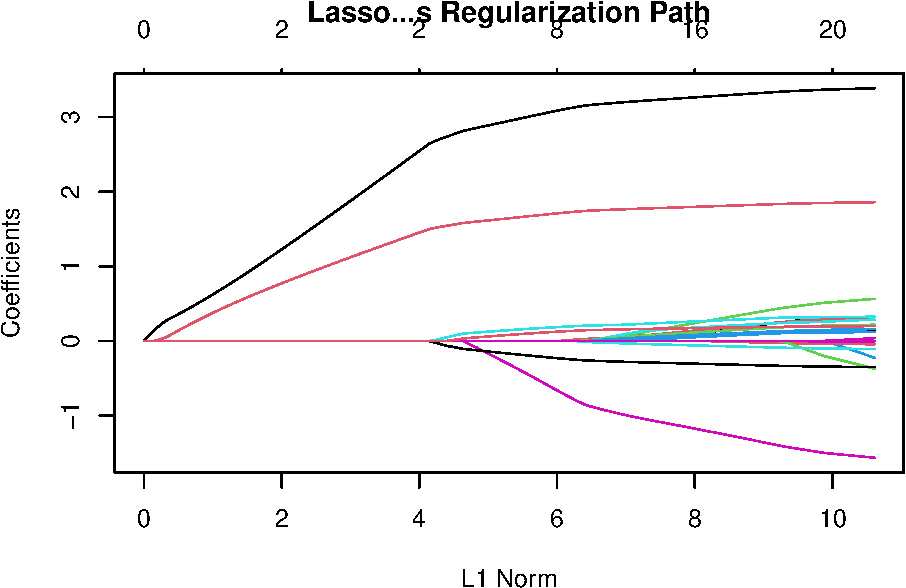
\includegraphics{HW3_Wu-Yulun_files/figure-latex/unnamed-chunk-2-1.pdf}

\begin{Shaded}
\begin{Highlighting}[]
\FunctionTok{plot}\NormalTok{(fit.ridge,}\AttributeTok{main=}\StringTok{"Ridge’s Regularization Path"}\NormalTok{,}\AttributeTok{xlab=}\StringTok{"L1 Norm"}\NormalTok{,}\AttributeTok{ylab=}\StringTok{"Coefficients"}\NormalTok{)}
\end{Highlighting}
\end{Shaded}

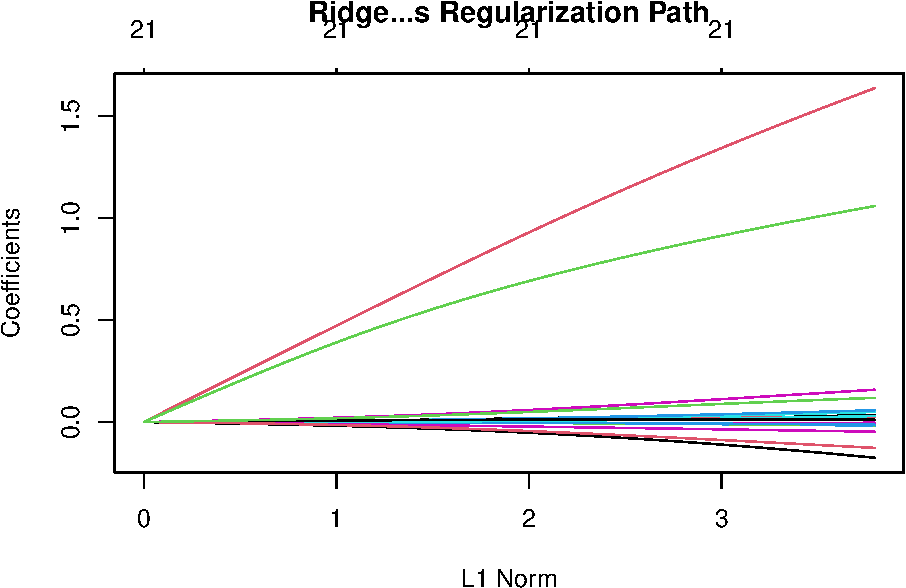
\includegraphics{HW3_Wu-Yulun_files/figure-latex/unnamed-chunk-2-2.pdf}

Part b

\begin{Shaded}
\begin{Highlighting}[]
\CommentTok{\# Coefficients of LASSO model in last column of beta}
\NormalTok{dim\_lassobeta }\OtherTok{=} \FunctionTok{dim}\NormalTok{(fit.lasso}\SpecialCharTok{$}\NormalTok{beta)}
\FunctionTok{abs}\NormalTok{(fit.lasso}\SpecialCharTok{$}\NormalTok{beta[,dim\_lassobeta[}\DecValTok{2}\NormalTok{]])}
\end{Highlighting}
\end{Shaded}

\begin{verbatim}
##          V1          V2          V3          V4          V5          V6 
## 0.328327302 0.316747742 0.564559336 0.223820136 0.288483703 0.038449854 
##          V7          V8          V9         V10         V11         V12 
## 0.138374944 0.000000000 0.043816121 0.369073039 0.121074354 0.325991793 
##         V13         V14         V15         V16         V17         V18 
## 1.563563657 3.386598177 1.859926722 0.218876930 0.159707350 0.107043787 
##         V19         V20         V21 
## 0.005933028 0.349789052 0.199048029
\end{verbatim}

\begin{Shaded}
\begin{Highlighting}[]
\CommentTok{\# Coefficients of Ridge model in last column of beta}
\NormalTok{dim\_ridgebeta }\OtherTok{=} \FunctionTok{dim}\NormalTok{(fit.ridge}\SpecialCharTok{$}\NormalTok{beta)}
\FunctionTok{abs}\NormalTok{(fit.ridge}\SpecialCharTok{$}\NormalTok{beta[,dim\_ridgebeta[}\DecValTok{2}\NormalTok{]])}
\end{Highlighting}
\end{Shaded}

\begin{verbatim}
##          V1          V2          V3          V4          V5          V6 
## 0.035307143 0.050432066 0.056810182 0.017564327 0.056305359 0.003434069 
##          V7          V8          V9         V10         V11         V12 
## 0.050430785 0.024361039 0.015590457 0.013324720 0.049368638 0.158586037 
##         V13         V14         V15         V16         V17         V18 
## 0.174961513 1.636953518 1.059298698 0.057802169 0.029305423 0.047219580 
##         V19         V20         V21 
## 0.011823948 0.126742968 0.118714798
\end{verbatim}

According to Google, the importance of features in LASSO and Ridge
Regression are indicated by the absolute value of corresponding
coefficient. The larger the absolute value of coefficient, the more
important the feature is.

In LASSO model, there are 3 features have coefficients such that the
absolute value of coefficient is greater than 1, ordering them in the
decreasing order of importance (absolute value of coefficients), they
are: Ad\_Width, Ad\_Height ,Domain=``trqRTuT-GNTYJNKbuKz''.

In Ridge model, there are 2 features have coefficients such that the
absolute value of coefficient is greater than 1, ordering them in the
decreasing order of importance (absolute value of coefficients), they
are: Ad\_Width, Ad\_Height.

Part c

\begin{Shaded}
\begin{Highlighting}[]
\CommentTok{\# Fit LASSO and Ridge 5 folds model}
\NormalTok{cv.lasso }\OtherTok{=} \FunctionTok{cv.glmnet}\NormalTok{(dataTrain,dataTrainAll}\SpecialCharTok{$}\NormalTok{Click,}\AttributeTok{family=}\StringTok{"binomial"}\NormalTok{,}\AttributeTok{standardize=}\ConstantTok{FALSE}\NormalTok{,}\AttributeTok{alpha=}\DecValTok{1}\NormalTok{,}\AttributeTok{nfolds =} \DecValTok{5}\NormalTok{)}

\NormalTok{cv.ridge }\OtherTok{=} \FunctionTok{cv.glmnet}\NormalTok{(dataTrain,dataTrainAll}\SpecialCharTok{$}\NormalTok{Click,}\AttributeTok{family=}\StringTok{"binomial"}\NormalTok{,}\AttributeTok{standardize=}\ConstantTok{FALSE}\NormalTok{,}\AttributeTok{alpha=}\DecValTok{0}\NormalTok{,}\AttributeTok{nfolds =} \DecValTok{5}\NormalTok{)}

\FunctionTok{par}\NormalTok{(}\AttributeTok{mfrow=}\FunctionTok{c}\NormalTok{(}\DecValTok{1}\NormalTok{,}\DecValTok{2}\NormalTok{))}
\FunctionTok{plot}\NormalTok{(fit.lasso,}\AttributeTok{main=}\StringTok{"Lasso’s Regularization Path"}\NormalTok{,}\AttributeTok{xlab=}\StringTok{"L1 Norm"}\NormalTok{,}\AttributeTok{ylab=}\StringTok{"Coefficients"}\NormalTok{)}
\FunctionTok{abline}\NormalTok{(}\AttributeTok{v=}\FunctionTok{sum}\NormalTok{(}\FunctionTok{abs}\NormalTok{(}\FunctionTok{coef}\NormalTok{(cv.lasso,}\AttributeTok{s=}\StringTok{"lambda.min"}\NormalTok{)[}\DecValTok{2}\SpecialCharTok{:}\DecValTok{22}\NormalTok{])))}
\FunctionTok{plot}\NormalTok{(cv.lasso,}\AttributeTok{main=}\StringTok{"Cross Validation for LASSO"}\NormalTok{,}\AttributeTok{xlab=}\StringTok{"log(Lambda)"}\NormalTok{,}\AttributeTok{ylab=}\StringTok{"Binomial Deviance"}\NormalTok{)}
\end{Highlighting}
\end{Shaded}

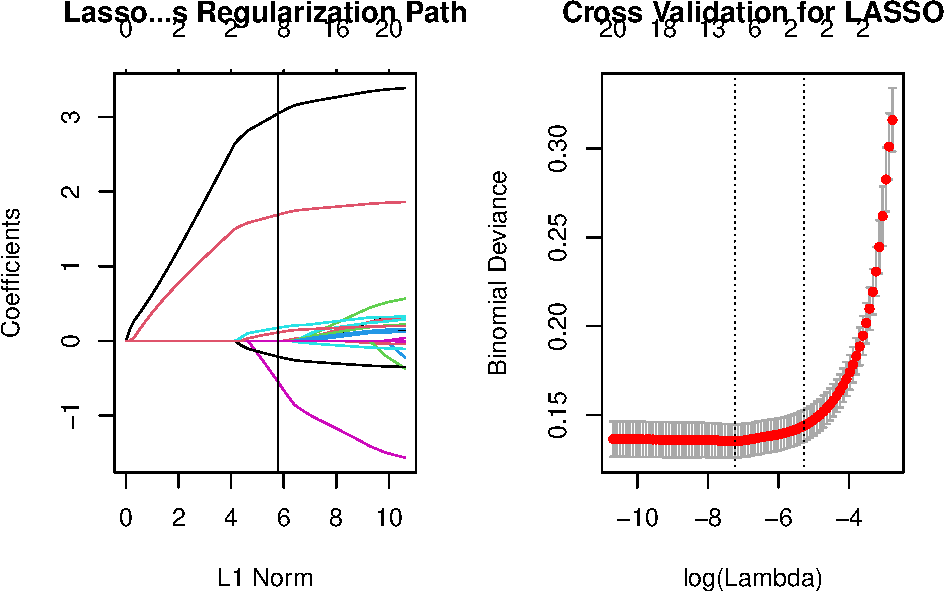
\includegraphics{HW3_Wu-Yulun_files/figure-latex/unnamed-chunk-4-1.pdf}

\begin{Shaded}
\begin{Highlighting}[]
\FunctionTok{par}\NormalTok{(}\AttributeTok{mfrow=}\FunctionTok{c}\NormalTok{(}\DecValTok{1}\NormalTok{,}\DecValTok{2}\NormalTok{))}
\FunctionTok{plot}\NormalTok{(fit.ridge,}\AttributeTok{main=}\StringTok{"Ridge’s Regularization Path"}\NormalTok{,}\AttributeTok{xlab=}\StringTok{"L1 Norm"}\NormalTok{,}\AttributeTok{ylab=}\StringTok{"Coefficients"}\NormalTok{)}
\FunctionTok{abline}\NormalTok{(}\AttributeTok{v=}\FunctionTok{sum}\NormalTok{(}\FunctionTok{abs}\NormalTok{(}\FunctionTok{coef}\NormalTok{(cv.ridge,}\AttributeTok{s=}\StringTok{"lambda.min"}\NormalTok{)[}\DecValTok{2}\SpecialCharTok{:}\DecValTok{22}\NormalTok{])))}
\FunctionTok{plot}\NormalTok{(cv.ridge,}\AttributeTok{main=}\StringTok{"Cross Validation for Ridge"}\NormalTok{,}\AttributeTok{xlab=}\StringTok{"log(Lambda)"}\NormalTok{,}\AttributeTok{ylab=}\StringTok{"Binomial Deviance"}\NormalTok{)}
\end{Highlighting}
\end{Shaded}

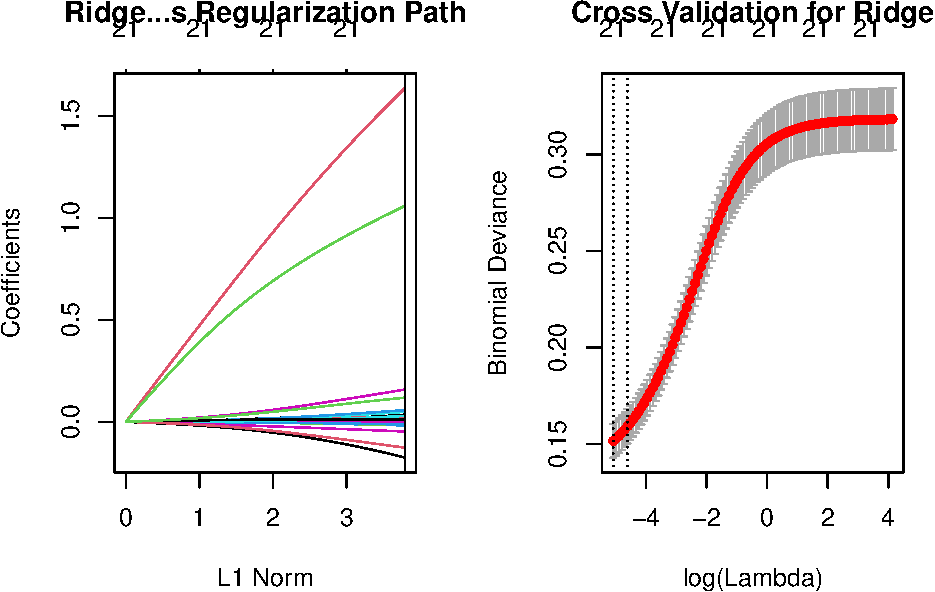
\includegraphics{HW3_Wu-Yulun_files/figure-latex/unnamed-chunk-4-2.pdf}
According to Part b and regularization path graph, 3 features play a
more important role in LASSO model when predicting whether there is at
least 1 click. The cross validation plot of LASSO Regression shows that
lambda that gives minimum cvm is around log(lambda)=-8, and the model
has around 16 non-zero features with lambda that gives minimum cvm.

According to Part b and regularization path graph, 2 features play a
more important role in Ridge model when predicting whether there is at
least 1 click. The cross validation plot of Ridge Regression shows that
lambda that gives minimum cvm is around log(lambda)=-5, and the model
has around 21 non-zero features with lambda that gives minimum cvm.

The reason why models with larger degrees of freedom do not necessarily
do better in the cross validation is because larger degrees of freedom
can cause overfitting, and models that overfit have higher cvm (mean
cross-validated error) in cross validation, and cross validation wants
to find a lambda such that cvm is minimized.

Part d

\begin{Shaded}
\begin{Highlighting}[]
\CommentTok{\# Modify dataTest in the way model wants}
\CommentTok{\# Create dummy variables}
\NormalTok{dataTest }\OtherTok{=} \FunctionTok{dummy\_cols}\NormalTok{(dataTest, }\AttributeTok{select\_columns =} \FunctionTok{c}\NormalTok{(}\StringTok{"Region"}\NormalTok{,}\StringTok{"City"}\NormalTok{,}\StringTok{"AdX"}\NormalTok{,}\StringTok{"Domain"}\NormalTok{,}\StringTok{"Key\_Page"}\NormalTok{,}\StringTok{"Ad\_Vis"}\NormalTok{,}\StringTok{"Ad\_Form"}\NormalTok{),}
\AttributeTok{remove\_first\_dummy =} \ConstantTok{TRUE}\NormalTok{, }\AttributeTok{ignore\_na =} \ConstantTok{TRUE}\NormalTok{, }\AttributeTok{remove\_selected\_columns =} \ConstantTok{FALSE}
\NormalTok{)}

\CommentTok{\# Column bind dummy variables}
\NormalTok{dataTest}\SpecialCharTok{$}\NormalTok{Region }\OtherTok{=} \FunctionTok{cbind}\NormalTok{(dataTest}\SpecialCharTok{$}\NormalTok{Region\_3,dataTest}\SpecialCharTok{$}\NormalTok{Region\_6)}
\NormalTok{dataTest}\SpecialCharTok{$}\NormalTok{City }\OtherTok{=} \FunctionTok{cbind}\NormalTok{(dataTest}\SpecialCharTok{$}\NormalTok{City\_2,dataTest}\SpecialCharTok{$}\NormalTok{City\_3,dataTest}\SpecialCharTok{$}\NormalTok{City\_4,dataTrainAll}\SpecialCharTok{$}\NormalTok{City\_5,dataTest}\SpecialCharTok{$}\NormalTok{City\_6)}
\NormalTok{dataTest}\SpecialCharTok{$}\NormalTok{AdX }\OtherTok{=} \FunctionTok{cbind}\NormalTok{(dataTest}\SpecialCharTok{$}\NormalTok{AdX\_2,dataTest}\SpecialCharTok{$}\NormalTok{AdX\_3)}
\NormalTok{dataTest}\SpecialCharTok{$}\NormalTok{Domain }\OtherTok{=} \FunctionTok{cbind}\NormalTok{(dataTest}\SpecialCharTok{$}\NormalTok{Domain\_5KFUl5p0Gxsvgmd4wspENpn,dataTest}\SpecialCharTok{$}\NormalTok{Domain\_trqRTu5Jg9q9wMKYvmpENpn,dataTest}\SpecialCharTok{$}\NormalTok{Domain\_trqRTudNXqN8ggc4JKTI,dataTest}\SpecialCharTok{$}\StringTok{\textasciigrave{}}\AttributeTok{Domain\_trqRTuT{-}GNTYJNKbuKz}\StringTok{\textasciigrave{}}\NormalTok{)}
\NormalTok{dataTest}\SpecialCharTok{$}\NormalTok{Key\_Page }\OtherTok{=} \FunctionTok{cbind}\NormalTok{(dataTest}\SpecialCharTok{$}\NormalTok{Key\_Page\_9f4e2f16b6873a7eb504df6f61b24044,dataTest}\SpecialCharTok{$}\NormalTok{Key\_Page\_df6f61b2409f4e2f16b6873a7eb50444)}
\NormalTok{dataTest}\SpecialCharTok{$}\NormalTok{Ad\_Vis }\OtherTok{=} \FunctionTok{cbind}\NormalTok{(dataTest}\SpecialCharTok{$}\NormalTok{Ad\_Vis\_1,dataTest}\SpecialCharTok{$}\NormalTok{Ad\_Vis\_2)}
\NormalTok{dataTest}\SpecialCharTok{$}\NormalTok{Ad\_Form }\OtherTok{=}\NormalTok{ dataTest}\SpecialCharTok{$}\NormalTok{Ad\_Form\_1}

\CommentTok{\# Standardized 3 columns}
\NormalTok{dataTest}\SpecialCharTok{$}\NormalTok{Ad\_Width }\OtherTok{=}\NormalTok{ (dataTest}\SpecialCharTok{$}\NormalTok{Ad\_Width }\SpecialCharTok{{-}} \FunctionTok{mean}\NormalTok{(dataTest}\SpecialCharTok{$}\NormalTok{Ad\_Width))}\SpecialCharTok{/}\FunctionTok{sd}\NormalTok{(dataTest}\SpecialCharTok{$}\NormalTok{Ad\_Width)}
\NormalTok{dataTest}\SpecialCharTok{$}\NormalTok{Ad\_Height }\OtherTok{=}\NormalTok{ (dataTest}\SpecialCharTok{$}\NormalTok{Ad\_Height }\SpecialCharTok{{-}} \FunctionTok{mean}\NormalTok{(dataTest}\SpecialCharTok{$}\NormalTok{Ad\_Height))}\SpecialCharTok{/}\FunctionTok{sd}\NormalTok{(dataTest}\SpecialCharTok{$}\NormalTok{Ad\_Height)}
\NormalTok{dataTest}\SpecialCharTok{$}\NormalTok{Floor\_Price }\OtherTok{=}\NormalTok{ (dataTest}\SpecialCharTok{$}\NormalTok{Floor\_Price }\SpecialCharTok{{-}} \FunctionTok{mean}\NormalTok{(dataTest}\SpecialCharTok{$}\NormalTok{Floor\_Price))}\SpecialCharTok{/}\FunctionTok{sd}\NormalTok{(dataTest}\SpecialCharTok{$}\NormalTok{Floor\_Price)}

\CommentTok{\# Put needed features in a dataframe}
\NormalTok{dataTest\_modified }\OtherTok{=} \FunctionTok{cbind}\NormalTok{(dataTest}\SpecialCharTok{$}\NormalTok{Region,dataTest}\SpecialCharTok{$}\NormalTok{City,dataTest}\SpecialCharTok{$}\NormalTok{AdX,dataTest}\SpecialCharTok{$}\NormalTok{Domain,dataTest}\SpecialCharTok{$}\NormalTok{Ad\_Width,dataTest}\SpecialCharTok{$}\NormalTok{Ad\_Height,dataTest}\SpecialCharTok{$}\NormalTok{Ad\_Vis,dataTest}\SpecialCharTok{$}\NormalTok{Ad\_Form,dataTest}\SpecialCharTok{$}\NormalTok{Floor\_Price,dataTest}\SpecialCharTok{$}\NormalTok{Key\_Page)}

\CommentTok{\# Modify Click column}
\NormalTok{dataTestRes}\SpecialCharTok{$}\NormalTok{Click[dataTestRes}\SpecialCharTok{$}\NormalTok{Click }\SpecialCharTok{\textgreater{}=} \DecValTok{1}\NormalTok{] }\OtherTok{=} \DecValTok{1}
\end{Highlighting}
\end{Shaded}

\begin{Shaded}
\begin{Highlighting}[]
\CommentTok{\# Number of rows in dataTestRes}
\NormalTok{n }\OtherTok{=} \FunctionTok{dim}\NormalTok{(dataTestRes)}
\NormalTok{n }\OtherTok{=}\NormalTok{ n[}\DecValTok{1}\NormalTok{]}
\CommentTok{\# Test for LASSO model}
\NormalTok{pred\_lasso }\OtherTok{=} \FunctionTok{predict}\NormalTok{(cv.lasso,dataTest\_modified,}\AttributeTok{s=}\StringTok{"lambda.min"}\NormalTok{)}
\NormalTok{predAndTruth.lasso }\OtherTok{=} \FunctionTok{cbind}\NormalTok{(pred\_lasso,dataTestRes}\SpecialCharTok{$}\NormalTok{Click) }\CommentTok{\# bind prediction and truth}
\CommentTok{\# True yi = 1, but prediction is 0}
\FunctionTok{nrow}\NormalTok{(predAndTruth.lasso[dataTestRes}\SpecialCharTok{$}\NormalTok{Click}\SpecialCharTok{==}\DecValTok{1}\SpecialCharTok{\&}\NormalTok{pred\_lasso}\SpecialCharTok{\textless{}}\DecValTok{0}\NormalTok{,])}\SpecialCharTok{/}\NormalTok{n}
\end{Highlighting}
\end{Shaded}

\begin{verbatim}
## [1] 0.0235
\end{verbatim}

\begin{Shaded}
\begin{Highlighting}[]
\CommentTok{\# True yi = 0, but prediction is 1}
\FunctionTok{nrow}\NormalTok{(predAndTruth.lasso[dataTestRes}\SpecialCharTok{$}\NormalTok{Click}\SpecialCharTok{==}\DecValTok{0}\SpecialCharTok{\&}\NormalTok{pred\_lasso}\SpecialCharTok{\textgreater{}}\DecValTok{0}\NormalTok{,])}\SpecialCharTok{/}\NormalTok{n}
\end{Highlighting}
\end{Shaded}

\begin{verbatim}
## [1] 0.0023
\end{verbatim}

\begin{Shaded}
\begin{Highlighting}[]
\CommentTok{\# Test for Ridge model}
\NormalTok{pred\_ridge }\OtherTok{=} \FunctionTok{predict}\NormalTok{(cv.ridge,dataTest\_modified,}\AttributeTok{s=}\StringTok{"lambda.min"}\NormalTok{)}
\NormalTok{predAndTruth.ridge }\OtherTok{=} \FunctionTok{cbind}\NormalTok{(pred\_ridge,dataTestRes}\SpecialCharTok{$}\NormalTok{Click) }\CommentTok{\# bind prediction and truth}
\CommentTok{\# True yi = 1, but prediction is 0}
\FunctionTok{nrow}\NormalTok{(predAndTruth.ridge[dataTestRes}\SpecialCharTok{$}\NormalTok{Click}\SpecialCharTok{==}\DecValTok{1}\SpecialCharTok{\&}\NormalTok{pred\_ridge}\SpecialCharTok{\textless{}}\DecValTok{0}\NormalTok{,])}\SpecialCharTok{/}\NormalTok{n}
\end{Highlighting}
\end{Shaded}

\begin{verbatim}
## [1] 0.0238
\end{verbatim}

\begin{Shaded}
\begin{Highlighting}[]
\CommentTok{\# True yi = 0, but prediction is 1}
\FunctionTok{nrow}\NormalTok{(predAndTruth.ridge[dataTestRes}\SpecialCharTok{$}\NormalTok{Click}\SpecialCharTok{==}\DecValTok{0}\SpecialCharTok{\&}\NormalTok{pred\_ridge}\SpecialCharTok{\textgreater{}}\DecValTok{0}\NormalTok{,])}\SpecialCharTok{/}\NormalTok{n}
\end{Highlighting}
\end{Shaded}

\begin{verbatim}
## [1] 0.002
\end{verbatim}

Q2

\begin{Shaded}
\begin{Highlighting}[]
\FunctionTok{load}\NormalTok{(}\StringTok{"q1.RData"}\NormalTok{)}

\CommentTok{\# Standardize 3 columns}
\NormalTok{dataTrainAll}\SpecialCharTok{$}\NormalTok{AdX }\OtherTok{=}\NormalTok{ (dataTrainAll}\SpecialCharTok{$}\NormalTok{AdX }\SpecialCharTok{{-}} \FunctionTok{mean}\NormalTok{(dataTrainAll}\SpecialCharTok{$}\NormalTok{AdX))}\SpecialCharTok{/}\FunctionTok{sd}\NormalTok{(dataTrainAll}\SpecialCharTok{$}\NormalTok{AdX)}
\NormalTok{dataTrainAll}\SpecialCharTok{$}\NormalTok{iPinYou\_Bid }\OtherTok{=}\NormalTok{ (dataTrainAll}\SpecialCharTok{$}\NormalTok{iPinYou\_Bid }\SpecialCharTok{{-}} \FunctionTok{mean}\NormalTok{(dataTrainAll}\SpecialCharTok{$}\NormalTok{iPinYou\_Bid))}\SpecialCharTok{/}\FunctionTok{sd}\NormalTok{(dataTrainAll}\SpecialCharTok{$}\NormalTok{iPinYou\_Bid)}
\NormalTok{dataTrainAll}\SpecialCharTok{$}\NormalTok{Comp\_Bid }\OtherTok{=}\NormalTok{ (dataTrainAll}\SpecialCharTok{$}\NormalTok{Comp\_Bid }\SpecialCharTok{{-}} \FunctionTok{mean}\NormalTok{(dataTrainAll}\SpecialCharTok{$}\NormalTok{Comp\_Bid))}\SpecialCharTok{/}\FunctionTok{sd}\NormalTok{(dataTrainAll}\SpecialCharTok{$}\NormalTok{Comp\_Bid)}
\NormalTok{dataTrain2 }\OtherTok{=} \FunctionTok{cbind}\NormalTok{(dataTrainAll}\SpecialCharTok{$}\NormalTok{AdX,dataTrainAll}\SpecialCharTok{$}\NormalTok{iPinYou\_Bid)}
\end{Highlighting}
\end{Shaded}

\begin{Shaded}
\begin{Highlighting}[]
\CommentTok{\# Fit linear model}
\NormalTok{fit.linear }\OtherTok{=} \FunctionTok{lm}\NormalTok{(Comp\_Bid}\SpecialCharTok{\textasciitilde{}}\NormalTok{AdX}\SpecialCharTok{+}\NormalTok{iPinYou\_Bid,}\AttributeTok{data=}\NormalTok{dataTrainAll)}
\NormalTok{fit.linear}\SpecialCharTok{$}\NormalTok{coefficients[}\DecValTok{2}\SpecialCharTok{:}\DecValTok{3}\NormalTok{] }\CommentTok{\# MLE coefficients of linear model}
\end{Highlighting}
\end{Shaded}

\begin{verbatim}
##         AdX iPinYou_Bid 
##  -0.1664490   0.7721763
\end{verbatim}

\begin{Shaded}
\begin{Highlighting}[]
\CommentTok{\# Fit LASSO model}
\NormalTok{fit.lasso }\OtherTok{=} \FunctionTok{glmnet}\NormalTok{(dataTrain2,dataTrainAll}\SpecialCharTok{$}\NormalTok{Comp\_Bid,}\AttributeTok{family=}\StringTok{"gaussian"}\NormalTok{,}\AttributeTok{standardize =} \ConstantTok{FALSE}\NormalTok{,}\AttributeTok{alpha=}\DecValTok{1}\NormalTok{)}
\NormalTok{half\_L1norm }\OtherTok{=} \FloatTok{0.5}\SpecialCharTok{*}\FunctionTok{sum}\NormalTok{(}\FunctionTok{abs}\NormalTok{(fit.linear}\SpecialCharTok{$}\NormalTok{coefficients[}\DecValTok{2}\SpecialCharTok{:}\DecValTok{3}\NormalTok{]))}
\NormalTok{half\_L1norm }\CommentTok{\# 0.5*L1 norm of MLE coefficients of linear model}
\end{Highlighting}
\end{Shaded}

\begin{verbatim}
## [1] 0.4693127
\end{verbatim}

\begin{Shaded}
\begin{Highlighting}[]
\NormalTok{beta\_leq\_half\_L1norm }\OtherTok{=}\NormalTok{ fit.lasso}\SpecialCharTok{$}\NormalTok{beta[,}\FunctionTok{colSums}\NormalTok{(}\FunctionTok{abs}\NormalTok{(fit.lasso}\SpecialCharTok{$}\NormalTok{beta))}\SpecialCharTok{\textless{}=}\NormalTok{half\_L1norm] }\CommentTok{\# All beta that have L1 norm \textless{}= half\_L1norm}
\NormalTok{lasso.coef }\OtherTok{=}\NormalTok{ beta\_leq\_half\_L1norm[,}\FunctionTok{dim}\NormalTok{(beta\_leq\_half\_L1norm)[}\DecValTok{2}\NormalTok{]] }\CommentTok{\# Beta that have max L1 norm among beta\_leq\_half\_L1norm}
\NormalTok{lasso.coef}
\end{Highlighting}
\end{Shaded}

\begin{verbatim}
##        V1        V2 
## 0.0000000 0.4382291
\end{verbatim}

\begin{Shaded}
\begin{Highlighting}[]
\NormalTok{beta1 }\OtherTok{=} \FunctionTok{seq}\NormalTok{(}\SpecialCharTok{{-}}\NormalTok{.}\DecValTok{5}\NormalTok{,}\DecValTok{1}\NormalTok{,}\AttributeTok{length.out=}\DecValTok{100}\NormalTok{)}
\NormalTok{beta2 }\OtherTok{=} \FunctionTok{seq}\NormalTok{(}\SpecialCharTok{{-}}\NormalTok{.}\DecValTok{5}\NormalTok{,}\DecValTok{1}\NormalTok{,}\AttributeTok{length.out=}\DecValTok{100}\NormalTok{)}
\NormalTok{beta }\OtherTok{=} \FunctionTok{expand.grid}\NormalTok{(beta1, beta2) }\CommentTok{\# Expand a grid of all combinations of beta1 and beta2}

\CommentTok{\# Function to calculate MSE of a single combination of beta1 and beta2}
\NormalTok{calc\_MSE }\OtherTok{=} \ControlFlowTok{function}\NormalTok{(beta1,beta2)\{}
  \FunctionTok{return}\NormalTok{(}\FunctionTok{sum}\NormalTok{((dataTrainAll}\SpecialCharTok{$}\NormalTok{Comp\_Bid}\SpecialCharTok{{-}}\NormalTok{beta1}\SpecialCharTok{*}\NormalTok{dataTrainAll}\SpecialCharTok{$}\NormalTok{AdX}\SpecialCharTok{{-}}\NormalTok{beta2}\SpecialCharTok{*}\NormalTok{dataTrainAll}\SpecialCharTok{$}\NormalTok{iPinYou\_Bid)}\SpecialCharTok{\^{}}\DecValTok{2}\NormalTok{))}
\NormalTok{\}}

\NormalTok{MSE }\OtherTok{=} \FunctionTok{mapply}\NormalTok{(calc\_MSE,beta[,}\DecValTok{1}\NormalTok{],beta[,}\DecValTok{2}\NormalTok{]) }\CommentTok{\# Use mapply to apply calc\_MSE to all combinations}
\NormalTok{MSE }\OtherTok{=} \FunctionTok{matrix}\NormalTok{(MSE,}\DecValTok{100}\NormalTok{,}\DecValTok{100}\NormalTok{)}
\NormalTok{L1\_lasso }\OtherTok{=} \FunctionTok{sum}\NormalTok{(}\FunctionTok{abs}\NormalTok{(lasso.coef))}
\FunctionTok{contour}\NormalTok{(beta1,beta2,MSE,}\AttributeTok{xlab=}\StringTok{"beta1"}\NormalTok{,}\AttributeTok{ylab=}\StringTok{"beta2"}\NormalTok{) }\CommentTok{\# Contour}
\FunctionTok{points}\NormalTok{(fit.linear}\SpecialCharTok{$}\NormalTok{coefficients[}\DecValTok{2}\NormalTok{],fit.linear}\SpecialCharTok{$}\NormalTok{coefficients[}\DecValTok{3}\NormalTok{],}\AttributeTok{col=}\StringTok{"red"}\NormalTok{) }\CommentTok{\# MLE coefficients}
\FunctionTok{points}\NormalTok{(lasso.coef[}\DecValTok{1}\NormalTok{],lasso.coef[}\DecValTok{2}\NormalTok{],}\AttributeTok{col=}\StringTok{"blue3"}\NormalTok{) }\CommentTok{\# LASSO coefficients}
\FunctionTok{plot}\NormalTok{(}\ControlFlowTok{function}\NormalTok{(x)\{x}\SpecialCharTok{+}\NormalTok{L1\_lasso\},}\SpecialCharTok{{-}}\NormalTok{L1\_lasso,}\DecValTok{0}\NormalTok{,}\AttributeTok{add=}\NormalTok{T,}\AttributeTok{col=}\StringTok{"green"}\NormalTok{)}
\FunctionTok{plot}\NormalTok{(}\ControlFlowTok{function}\NormalTok{(x)\{}\SpecialCharTok{{-}}\NormalTok{x}\SpecialCharTok{{-}}\NormalTok{L1\_lasso\},}\SpecialCharTok{{-}}\NormalTok{L1\_lasso,}\DecValTok{0}\NormalTok{,}\AttributeTok{add=}\NormalTok{T,}\AttributeTok{col=}\StringTok{"green"}\NormalTok{)}
\FunctionTok{plot}\NormalTok{(}\ControlFlowTok{function}\NormalTok{(x)\{x}\SpecialCharTok{{-}}\NormalTok{L1\_lasso\},}\DecValTok{0}\NormalTok{,L1\_lasso,}\AttributeTok{add=}\NormalTok{T,}\AttributeTok{col=}\StringTok{"green"}\NormalTok{)}
\FunctionTok{plot}\NormalTok{(}\ControlFlowTok{function}\NormalTok{(x)\{}\SpecialCharTok{{-}}\NormalTok{x}\SpecialCharTok{+}\NormalTok{L1\_lasso\},}\DecValTok{0}\NormalTok{,L1\_lasso,}\AttributeTok{add=}\NormalTok{T,}\AttributeTok{col=}\StringTok{"green"}\NormalTok{)}
\end{Highlighting}
\end{Shaded}

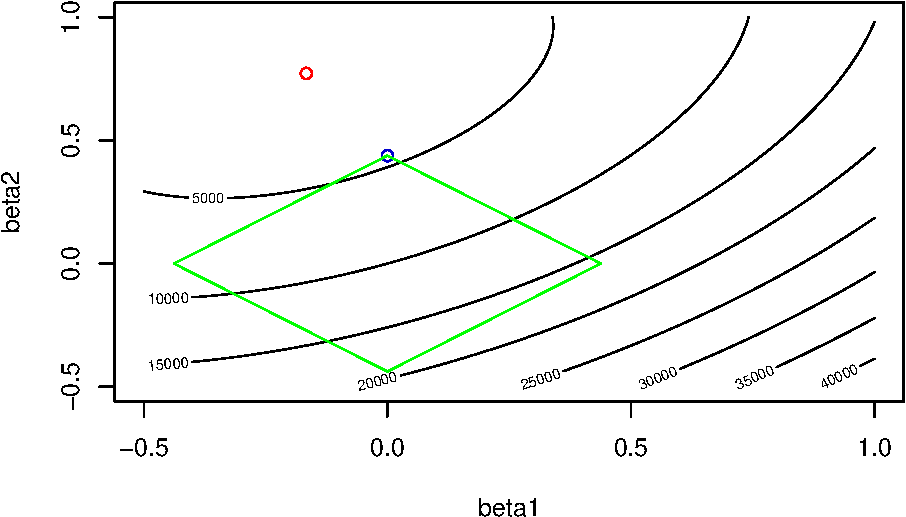
\includegraphics{HW3_Wu-Yulun_files/figure-latex/unnamed-chunk-8-1.pdf}

\begin{Shaded}
\begin{Highlighting}[]
\CommentTok{\# Ridge Regression part}
\FunctionTok{library}\NormalTok{(wordspace)}
\FunctionTok{library}\NormalTok{(DescTools)}
\NormalTok{fit.ridge }\OtherTok{=} \FunctionTok{glmnet}\NormalTok{(dataTrain2,dataTrainAll}\SpecialCharTok{$}\NormalTok{Comp\_Bid,}\AttributeTok{family=}\StringTok{"gaussian"}\NormalTok{,}\AttributeTok{standardize=}\ConstantTok{FALSE}\NormalTok{,}\AttributeTok{alpha=}\DecValTok{0}\NormalTok{)}
\NormalTok{half\_L2norm }\OtherTok{=} \FloatTok{0.5}\SpecialCharTok{*}\FunctionTok{norm}\NormalTok{(fit.linear}\SpecialCharTok{$}\NormalTok{coefficients[}\DecValTok{2}\SpecialCharTok{:}\DecValTok{3}\NormalTok{], }\AttributeTok{type =} \StringTok{"2"}\NormalTok{)   }
\NormalTok{half\_L2norm }\CommentTok{\# 0.5*L2 norm of MLE coefficients of linear model}
\end{Highlighting}
\end{Shaded}

\begin{verbatim}
## [1] 0.3949562
\end{verbatim}

\begin{Shaded}
\begin{Highlighting}[]
\NormalTok{beta\_leq\_half\_L2norm }\OtherTok{=}\NormalTok{ fit.ridge}\SpecialCharTok{$}\NormalTok{beta[,}\FunctionTok{colNorms}\NormalTok{(fit.ridge}\SpecialCharTok{$}\NormalTok{beta)}\SpecialCharTok{\textless{}=}\NormalTok{half\_L2norm] }\CommentTok{\# All beta that have L2 norm \textless{}= half\_L2norm}
\NormalTok{ridge.coef }\OtherTok{=}\NormalTok{ beta\_leq\_half\_L2norm[,}\FunctionTok{dim}\NormalTok{(beta\_leq\_half\_L2norm)[}\DecValTok{2}\NormalTok{]] }\CommentTok{\# Beta that have max L2 norm among beta\_leq\_half\_L2norm}
\NormalTok{ridge.coef}
\end{Highlighting}
\end{Shaded}

\begin{verbatim}
##         V1         V2 
## -0.1455805  0.3482623
\end{verbatim}

\begin{Shaded}
\begin{Highlighting}[]
\NormalTok{L2\_ridge }\OtherTok{=} \FunctionTok{norm}\NormalTok{(ridge.coef, }\AttributeTok{type =} \StringTok{"2"}\NormalTok{) }
\FunctionTok{contour}\NormalTok{(beta1,beta2,MSE,}\AttributeTok{xlab=}\StringTok{"beta1"}\NormalTok{,}\AttributeTok{ylab=}\StringTok{"beta2"}\NormalTok{) }\CommentTok{\# Contour}
\FunctionTok{points}\NormalTok{(fit.linear}\SpecialCharTok{$}\NormalTok{coefficients[}\DecValTok{2}\NormalTok{],fit.linear}\SpecialCharTok{$}\NormalTok{coefficients[}\DecValTok{3}\NormalTok{],}\AttributeTok{col=}\StringTok{"red"}\NormalTok{) }\CommentTok{\# MLE coefficients}
\FunctionTok{points}\NormalTok{(ridge.coef[}\DecValTok{1}\NormalTok{],ridge.coef[}\DecValTok{2}\NormalTok{],}\AttributeTok{col=}\StringTok{"blue3"}\NormalTok{) }\CommentTok{\# Ridge coefficients}
\FunctionTok{DrawEllipse}\NormalTok{(}\DecValTok{0}\NormalTok{,}\DecValTok{0}\NormalTok{, }\AttributeTok{radius.x =}\NormalTok{ L2\_ridge, }\AttributeTok{radius.y =}\NormalTok{ L2\_ridge,}\AttributeTok{border=}\StringTok{"green"}\NormalTok{,}\AttributeTok{col =}\ConstantTok{NA}\NormalTok{)}
\end{Highlighting}
\end{Shaded}

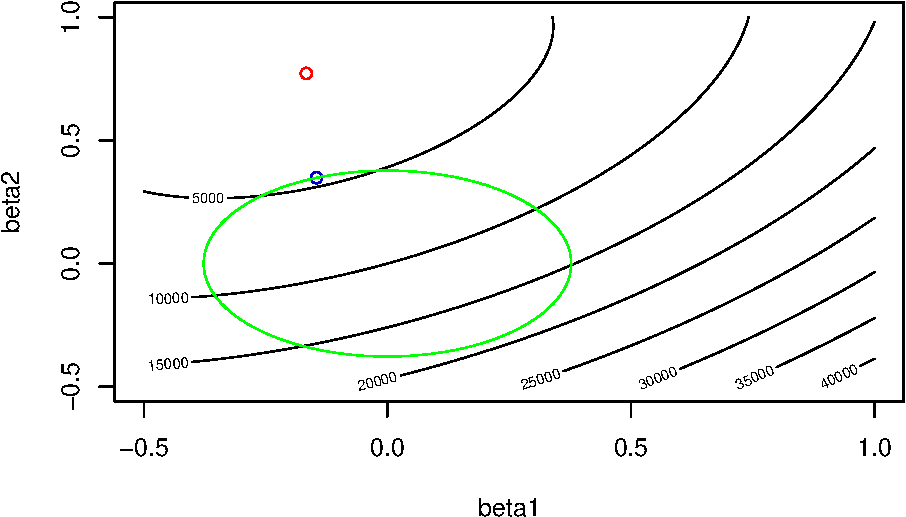
\includegraphics{HW3_Wu-Yulun_files/figure-latex/unnamed-chunk-8-2.pdf}
The MLE coefficients sit at the center of the level curve. MLE
coefficients minimize MSE. LASSO and Ridge coefficients sit close to the
most inner contour curve (5000), It is the point on L1 or L2 ball that
has minimum MSE. LASSO and Ridge try to minimize MSE while coefficients
satisfy L1/L2 norm. LASSO encourages sparse because L1 ball is diamond
shape, so the L1 diamond have greater chance to have minimum MSE at 4
corner point, and at corner point, there is one coefficient equal to 0
(in 2d case). A simple example is, when you rotate a circle for 360
degree, during the rotation, any point on circle can be a maximum point
at some angle with equal occurrence; but if you rotate a diamond, 4
corner point have further higher frequency to become maximum points than
others.

\hypertarget{question-5-20-points-discover-gravitational-waves-in-your-room}{%
\subsection{Question 5 (20 Points) Discover Gravitational Waves in Your
Room}\label{question-5-20-points-discover-gravitational-waves-in-your-room}}

\hypertarget{answer-1}{%
\subsubsection{Answer:}\label{answer-1}}

\begin{Shaded}
\begin{Highlighting}[]
\FunctionTok{set.seed}\NormalTok{(}\DecValTok{10}\NormalTok{)}
\NormalTok{LIGO }\OtherTok{=} \FunctionTok{read.table}\NormalTok{(}\StringTok{"LIGO.Hanford.Data.txt"}\NormalTok{, }\AttributeTok{header=}\NormalTok{F)}
\FunctionTok{head}\NormalTok{(LIGO)}
\end{Highlighting}
\end{Shaded}

\begin{verbatim}
##          V1           V2
## 1 0.2500000  0.026422536
## 2 0.2500610 -0.003132572
## 3 0.2501221 -0.130760718
## 4 0.2501831 -0.061991781
## 5 0.2502441  0.019565419
## 6 0.2503052  0.022075875
\end{verbatim}

Q1

\begin{Shaded}
\begin{Highlighting}[]
\NormalTok{n\_row }\OtherTok{=} \FunctionTok{nrow}\NormalTok{(LIGO)}
\NormalTok{sqrt\_n\_row }\OtherTok{=} \FunctionTok{sqrt}\NormalTok{(n\_row)}
\NormalTok{C }\OtherTok{=} \FunctionTok{matrix}\NormalTok{(, }\AttributeTok{nrow =}\NormalTok{ n\_row, }\AttributeTok{ncol =}\NormalTok{ n\_row)}
\ControlFlowTok{for}\NormalTok{ (j }\ControlFlowTok{in} \DecValTok{1}\SpecialCharTok{:}\NormalTok{n\_row)\{}
  \ControlFlowTok{for}\NormalTok{ (k }\ControlFlowTok{in} \DecValTok{1}\SpecialCharTok{:}\NormalTok{n\_row)\{}
    \ControlFlowTok{if}\NormalTok{ (j}\SpecialCharTok{==}\DecValTok{1}\NormalTok{)\{}
\NormalTok{      C[j,k] }\OtherTok{=}\NormalTok{ sqrt\_n\_row}
\NormalTok{    \}}
    \ControlFlowTok{else}\NormalTok{ \{}
\NormalTok{      C[j,k] }\OtherTok{=} \FunctionTok{sqrt}\NormalTok{(}\DecValTok{2}\SpecialCharTok{/}\NormalTok{n\_row)}\SpecialCharTok{*}\FunctionTok{cos}\NormalTok{(pi}\SpecialCharTok{*}\NormalTok{(}\DecValTok{2}\SpecialCharTok{*}\NormalTok{k}\DecValTok{{-}1}\NormalTok{)}\SpecialCharTok{*}\NormalTok{(j}\DecValTok{{-}1}\NormalTok{)}\SpecialCharTok{/}\NormalTok{(}\DecValTok{2}\SpecialCharTok{*}\NormalTok{n\_row))}
\NormalTok{    \}}
\NormalTok{  \}}
\NormalTok{\}}

\NormalTok{cv.lasso }\OtherTok{=} \FunctionTok{cv.glmnet}\NormalTok{(C,}\FunctionTok{as.matrix}\NormalTok{(LIGO[}\DecValTok{2}\NormalTok{]),}\AttributeTok{alpha=}\DecValTok{1}\NormalTok{,}\AttributeTok{nfolds =} \DecValTok{10}\NormalTok{)}
\CommentTok{\#w\_hat = cv.lasso$beta[,cv.lasso$lambda.min]}
\CommentTok{\#cv.lasso$beta}
\NormalTok{y\_pred }\OtherTok{=} \FunctionTok{predict}\NormalTok{(cv.lasso,C,}\AttributeTok{s=}\StringTok{"lambda.min"}\NormalTok{)}
\CommentTok{\#plot(cv.lasso$beta,)}
\NormalTok{cv.lasso}\SpecialCharTok{$}\NormalTok{beta}
\end{Highlighting}
\end{Shaded}

Q2

\hypertarget{question-6-25-points-upright-human-detection-in-photos}{%
\subsection{Question 6 (25 Points) Upright Human Detection in
Photos}\label{question-6-25-points-upright-human-detection-in-photos}}

\hypertarget{answer-2}{%
\subsubsection{Answer:}\label{answer-2}}

\begin{enumerate}
\def\labelenumi{(\alph{enumi})}
\tightlist
\item
\end{enumerate}

\begin{Shaded}
\begin{Highlighting}[]
\FunctionTok{library}\NormalTok{(png)}
\FunctionTok{source}\NormalTok{(}\StringTok{"functions.R"}\NormalTok{)}
\NormalTok{subdir\_pos }\OtherTok{=} \StringTok{"/pngdata/pos/"}
\NormalTok{subdir\_neg }\OtherTok{=} \StringTok{"/pngdata/neg/"}
\NormalTok{filename\_pos }\OtherTok{=} \StringTok{"5"}
\NormalTok{filename\_neg }\OtherTok{=} \StringTok{"7"}
\NormalTok{photo\_pos }\OtherTok{=} \FunctionTok{readPNG}\NormalTok{(}\FunctionTok{paste}\NormalTok{(}\FunctionTok{file.path}\NormalTok{(}\FunctionTok{getwd}\NormalTok{(),subdir\_pos,filename\_pos), }\StringTok{".png"}\NormalTok{, }\AttributeTok{sep =} \StringTok{""}\NormalTok{))}
\NormalTok{photo\_neg }\OtherTok{=} \FunctionTok{readPNG}\NormalTok{(}\FunctionTok{paste}\NormalTok{(}\FunctionTok{file.path}\NormalTok{(}\FunctionTok{getwd}\NormalTok{(),subdir\_neg,filename\_neg), }\StringTok{".png"}\NormalTok{, }\AttributeTok{sep =} \StringTok{""}\NormalTok{))}
\CommentTok{\# Transfer to the black and white version}
\NormalTok{photo\_pos }\OtherTok{=} \FunctionTok{rgb2gray}\NormalTok{(photo\_pos)}
\FunctionTok{writePNG}\NormalTok{(photo\_pos, }\AttributeTok{target =} \StringTok{"bwpos.png"}\NormalTok{)}
\NormalTok{photo\_neg }\OtherTok{=} \FunctionTok{rgb2gray}\NormalTok{(photo\_neg)}
\FunctionTok{writePNG}\NormalTok{(photo\_neg, }\AttributeTok{target =} \StringTok{"bwneg.png"}\NormalTok{)}

\NormalTok{photo\_neg }\OtherTok{=} \FunctionTok{crop.r}\NormalTok{(photo\_neg,}\DecValTok{160}\NormalTok{,}\DecValTok{96}\NormalTok{) }\CommentTok{\# Randomly crop}
\FunctionTok{writePNG}\NormalTok{(photo\_neg, }\AttributeTok{target =} \StringTok{"cropneg.png"}\NormalTok{)}

\NormalTok{photo\_pos.grad }\OtherTok{=} \FunctionTok{grad}\NormalTok{(photo\_pos, }\DecValTok{128}\NormalTok{, }\DecValTok{64}\NormalTok{, F)}
\FunctionTok{setEPS}\NormalTok{()}
\FunctionTok{postscript}\NormalTok{(}\StringTok{"gradpos.eps"}\NormalTok{)}
\NormalTok{g}\OtherTok{=}\FunctionTok{grad}\NormalTok{(photo\_pos, }\DecValTok{128}\NormalTok{, }\DecValTok{64}\NormalTok{, T)}
\FunctionTok{dev.off}\NormalTok{()}
\end{Highlighting}
\end{Shaded}

\begin{verbatim}
## pdf 
##   2
\end{verbatim}

\begin{Shaded}
\begin{Highlighting}[]
\NormalTok{photo\_neg.grad }\OtherTok{=} \FunctionTok{grad}\NormalTok{(photo\_neg, }\DecValTok{128}\NormalTok{, }\DecValTok{64}\NormalTok{, F)}
\FunctionTok{setEPS}\NormalTok{()}
\FunctionTok{postscript}\NormalTok{(}\StringTok{"gradneg.eps"}\NormalTok{)}
\NormalTok{g}\OtherTok{=}\FunctionTok{grad}\NormalTok{(photo\_neg, }\DecValTok{128}\NormalTok{, }\DecValTok{64}\NormalTok{, T)}
\FunctionTok{dev.off}\NormalTok{()}
\end{Highlighting}
\end{Shaded}

\begin{verbatim}
## pdf 
##   2
\end{verbatim}

\begin{Shaded}
\begin{Highlighting}[]
\NormalTok{photo\_pos.hog }\OtherTok{=} \FunctionTok{hog}\NormalTok{(photo\_pos.grad}\SpecialCharTok{$}\NormalTok{xgrad, photo\_pos.grad}\SpecialCharTok{$}\NormalTok{ygrad, }\DecValTok{4}\NormalTok{, }\DecValTok{4}\NormalTok{, }\DecValTok{6}\NormalTok{)}
\NormalTok{photo\_neg.hog }\OtherTok{=} \FunctionTok{hog}\NormalTok{(photo\_neg.grad}\SpecialCharTok{$}\NormalTok{xgrad, photo\_neg.grad}\SpecialCharTok{$}\NormalTok{ygrad, }\DecValTok{4}\NormalTok{, }\DecValTok{4}\NormalTok{, }\DecValTok{6}\NormalTok{)}
\end{Highlighting}
\end{Shaded}

\includegraphics[width=0.8\linewidth]{pngdata/pos/5}
\includegraphics[width=0.8\linewidth]{bwpos}
\includegraphics[width=0.8\linewidth]{gradpos}

\begin{verbatim}
##  [1] 0.23828125 0.45312500 0.10156250 0.02148438 0.07031250 0.05273438
##  [7] 0.10546875 0.17773438 0.13281250 0.12109375 0.27148438 0.18945312
## [13] 0.13281250 0.25585938 0.11328125 0.13085938 0.25585938 0.11132812
## [19] 0.13085938 0.20703125 0.14062500 0.09179688 0.32617188 0.08789062
## [25] 0.25781250 0.12500000 0.21289062 0.12109375 0.13867188 0.14453125
## [31] 0.16406250 0.10937500 0.15429688 0.16406250 0.11328125 0.29296875
## [37] 0.22656250 0.26367188 0.14453125 0.10546875 0.11328125 0.14453125
## [43] 0.23632812 0.21093750 0.14453125 0.11132812 0.19531250 0.10156250
## [49] 0.20117188 0.32226562 0.13085938 0.10546875 0.11132812 0.06445312
## [55] 0.07421875 0.10937500 0.33203125 0.29296875 0.10156250 0.08984375
## [61] 0.13085938 0.19531250 0.22851562 0.20117188 0.16796875 0.07617188
## [67] 0.22070312 0.22656250 0.19726562 0.10937500 0.16601562 0.08007812
## [73] 0.18164062 0.40820312 0.11718750 0.03906250 0.15625000 0.03515625
## [79] 0.05273438 0.21484375 0.06640625 0.11523438 0.41992188 0.13085938
## [85] 0.05078125 0.40234375 0.05664062 0.04492188 0.36718750 0.07812500
## [91] 0.13281250 0.17968750 0.08593750 0.08007812 0.41992188 0.07031250
\end{verbatim}

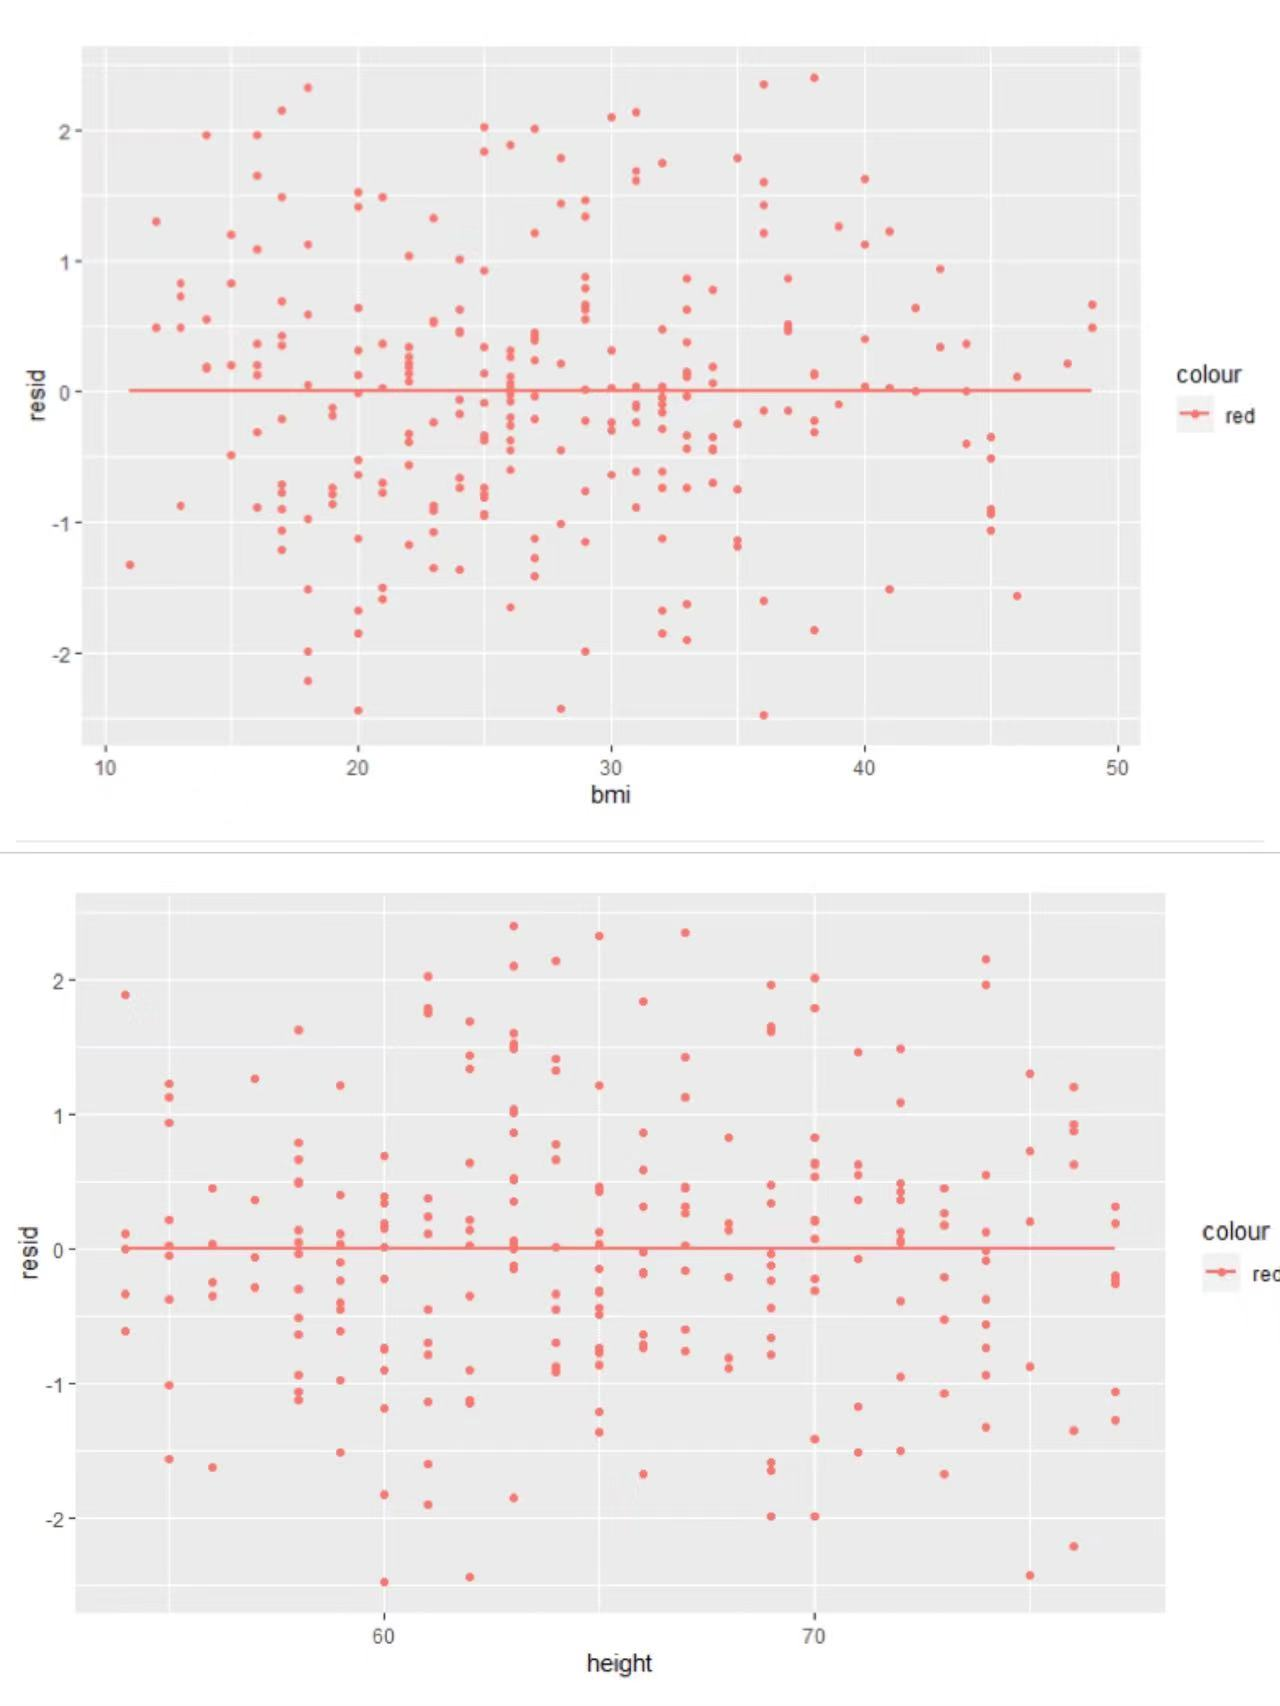
\includegraphics[width=0.8\linewidth]{pngdata/neg/7}
\includegraphics[width=0.8\linewidth]{bwneg}
\includegraphics[width=0.8\linewidth]{cropneg}
\includegraphics[width=0.8\linewidth]{gradneg}

\begin{verbatim}
##  [1] 0.18359375 0.15625000 0.16406250 0.19335938 0.16406250 0.13867188
##  [7] 0.21289062 0.16992188 0.12695312 0.18750000 0.16796875 0.13476562
## [13] 0.15234375 0.10937500 0.23828125 0.21875000 0.11914062 0.16210938
## [19] 0.15234375 0.19335938 0.24414062 0.16796875 0.10742188 0.13476562
## [25] 0.18164062 0.16015625 0.16406250 0.18554688 0.16406250 0.14453125
## [31] 0.18750000 0.17187500 0.15625000 0.18359375 0.15234375 0.14843750
## [37] 0.11523438 0.16015625 0.16210938 0.22070312 0.17578125 0.16601562
## [43] 0.16406250 0.22851562 0.22656250 0.14257812 0.12695312 0.11132812
## [49] 0.14843750 0.14257812 0.17773438 0.20898438 0.19335938 0.12890625
## [55] 0.12304688 0.17578125 0.20507812 0.27148438 0.11718750 0.10742188
## [61] 0.07812500 0.20117188 0.23046875 0.17578125 0.21093750 0.10351562
## [67] 0.11914062 0.24804688 0.18359375 0.16406250 0.17578125 0.10937500
## [73] 0.15820312 0.16406250 0.16015625 0.16601562 0.17773438 0.17382812
## [79] 0.26757812 0.12109375 0.15820312 0.08593750 0.10546875 0.26171875
## [85] 0.16210938 0.09570312 0.25390625 0.18164062 0.08593750 0.22070312
## [91] 0.11718750 0.24609375 0.27929688 0.13085938 0.11718750 0.10937500
\end{verbatim}

\begin{enumerate}
\def\labelenumi{(\alph{enumi})}
\setcounter{enumi}{1}
\tightlist
\item
\end{enumerate}

\begin{Shaded}
\begin{Highlighting}[]
\FunctionTok{getwd}\NormalTok{()}
\end{Highlighting}
\end{Shaded}

\begin{verbatim}
## [1] "/Users/yulunwu/Downloads/2023winter/STAD80/A3"
\end{verbatim}

\begin{Shaded}
\begin{Highlighting}[]
\NormalTok{n}\OtherTok{=}\DecValTok{500}
\NormalTok{features\_pos }\OtherTok{=} \FunctionTok{data.frame}\NormalTok{(}\FunctionTok{matrix}\NormalTok{(}\AttributeTok{ncol =} \DecValTok{96}\NormalTok{, }\AttributeTok{nrow =} \DecValTok{0}\NormalTok{))}
\NormalTok{features\_neg }\OtherTok{=} \FunctionTok{data.frame}\NormalTok{(}\FunctionTok{matrix}\NormalTok{(}\AttributeTok{ncol =} \DecValTok{96}\NormalTok{, }\AttributeTok{nrow =} \DecValTok{0}\NormalTok{))}
\ControlFlowTok{for}\NormalTok{ (i }\ControlFlowTok{in} \DecValTok{1}\SpecialCharTok{:}\DecValTok{500}\NormalTok{)\{}
\NormalTok{  photo\_pos }\OtherTok{=} \FunctionTok{readPNG}\NormalTok{(}\FunctionTok{paste}\NormalTok{(}\FunctionTok{file.path}\NormalTok{(}\FunctionTok{getwd}\NormalTok{(),subdir\_pos,}\FunctionTok{as.character}\NormalTok{(i)), }\StringTok{".png"}\NormalTok{, }\AttributeTok{sep =} \StringTok{""}\NormalTok{))}
\NormalTok{  photo\_neg }\OtherTok{=} \FunctionTok{readPNG}\NormalTok{(}\FunctionTok{paste}\NormalTok{(}\FunctionTok{file.path}\NormalTok{(}\FunctionTok{getwd}\NormalTok{(),subdir\_neg,}\FunctionTok{as.character}\NormalTok{(i)), }\StringTok{".png"}\NormalTok{, }\AttributeTok{sep =} \StringTok{""}\NormalTok{))}
  \CommentTok{\# Transfer to the black and white version}
\NormalTok{  photo\_pos }\OtherTok{=} \FunctionTok{rgb2gray}\NormalTok{(photo\_pos)}
\NormalTok{  photo\_neg }\OtherTok{=} \FunctionTok{rgb2gray}\NormalTok{(photo\_neg)}
  
\NormalTok{  photo\_neg }\OtherTok{=} \FunctionTok{crop.r}\NormalTok{(photo\_neg,}\DecValTok{160}\NormalTok{,}\DecValTok{96}\NormalTok{) }\CommentTok{\# Randomly crop}

\NormalTok{  photo\_pos.grad }\OtherTok{=} \FunctionTok{grad}\NormalTok{(photo\_pos, }\DecValTok{128}\NormalTok{, }\DecValTok{64}\NormalTok{, F)}
\NormalTok{  photo\_neg.grad }\OtherTok{=} \FunctionTok{grad}\NormalTok{(photo\_neg, }\DecValTok{128}\NormalTok{, }\DecValTok{64}\NormalTok{, F)}

\NormalTok{  photo\_pos.hog }\OtherTok{=} \FunctionTok{hog}\NormalTok{(photo\_pos.grad}\SpecialCharTok{$}\NormalTok{xgrad, photo\_pos.grad}\SpecialCharTok{$}\NormalTok{ygrad, }\DecValTok{4}\NormalTok{, }\DecValTok{4}\NormalTok{, }\DecValTok{6}\NormalTok{)}
\NormalTok{  photo\_neg.hog }\OtherTok{=} \FunctionTok{hog}\NormalTok{(photo\_neg.grad}\SpecialCharTok{$}\NormalTok{xgrad, photo\_neg.grad}\SpecialCharTok{$}\NormalTok{ygrad, }\DecValTok{4}\NormalTok{, }\DecValTok{4}\NormalTok{, }\DecValTok{6}\NormalTok{)}
  
\NormalTok{  features\_pos[i,] }\OtherTok{=}\NormalTok{ photo\_pos.hog}
\NormalTok{  features\_neg[i,] }\OtherTok{=}\NormalTok{ photo\_neg.hog}
\NormalTok{\}}
\NormalTok{features\_data }\OtherTok{=} \FunctionTok{rbind}\NormalTok{(features\_pos,features\_neg) }\CommentTok{\# Row bind two dataframe together, row 1 to 500 are POS, 501 to 1000 are NEG}
\NormalTok{features\_data[}\DecValTok{1}\SpecialCharTok{:}\DecValTok{500}\NormalTok{,}\StringTok{"POS"}\NormalTok{] }\OtherTok{=} \DecValTok{1} \CommentTok{\# 1 indicates POS}
\NormalTok{features\_data[}\DecValTok{501}\SpecialCharTok{:}\DecValTok{1000}\NormalTok{,}\StringTok{"POS"}\NormalTok{] }\OtherTok{=} \DecValTok{0} \CommentTok{\# 0 indicates NEG}
\end{Highlighting}
\end{Shaded}

Part II

\begin{Shaded}
\begin{Highlighting}[]
\NormalTok{fit.logit }\OtherTok{=} \FunctionTok{glmnet}\NormalTok{(features\_data[,}\DecValTok{1}\SpecialCharTok{:}\DecValTok{96}\NormalTok{],features\_data}\SpecialCharTok{$}\NormalTok{POS,}\AttributeTok{family=}\StringTok{"binomial"}\NormalTok{)}
\FunctionTok{plot}\NormalTok{(fit.logit,}\AttributeTok{main=}\StringTok{"Logistic\textquotesingle{}s Regularization Path"}\NormalTok{,}\AttributeTok{xlab=}\StringTok{""}\NormalTok{,}\AttributeTok{ylab=}\StringTok{"Coefficients"}\NormalTok{)}
\end{Highlighting}
\end{Shaded}

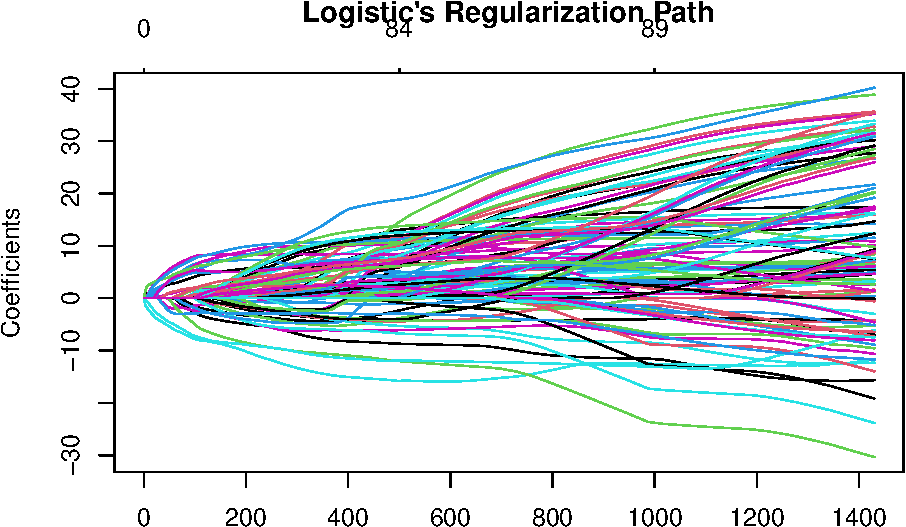
\includegraphics{HW3_Wu-Yulun_files/figure-latex/unnamed-chunk-14-1.pdf}

\begin{Shaded}
\begin{Highlighting}[]
\NormalTok{fit.logit.cv }\OtherTok{=} \FunctionTok{cv.glmnet}\NormalTok{(}\FunctionTok{as.matrix}\NormalTok{(features\_data[,}\DecValTok{1}\SpecialCharTok{:}\DecValTok{96}\NormalTok{]),features\_data}\SpecialCharTok{$}\NormalTok{POS,}\AttributeTok{family=}\StringTok{"binomial"}\NormalTok{,}\AttributeTok{type.measure=}\StringTok{"class"}\NormalTok{)}
\FunctionTok{plot}\NormalTok{(fit.logit.cv,}\AttributeTok{main=}\StringTok{"Cross Validation for Logistic"}\NormalTok{,}\AttributeTok{xlab=}\StringTok{"Lambda"}\NormalTok{,}\AttributeTok{ylab=}\StringTok{"Cross Validation Errors (CVM)"}\NormalTok{)}
\end{Highlighting}
\end{Shaded}

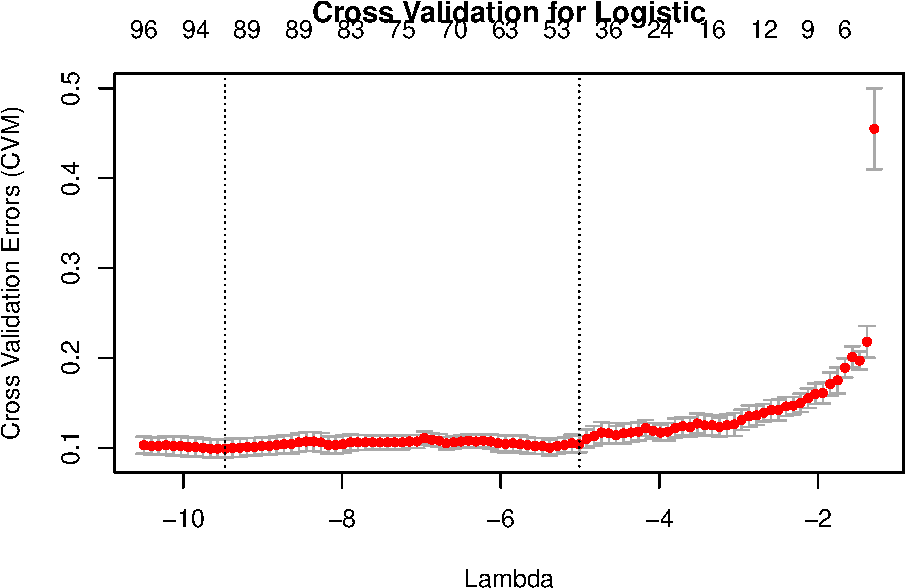
\includegraphics{HW3_Wu-Yulun_files/figure-latex/unnamed-chunk-14-2.pdf}

\hypertarget{question-7-30-points-sentiment-analysis-on-amazon-product-reviews}{%
\subsection{Question 7 (30 Points) Sentiment Analysis on Amazon Product
Reviews}\label{question-7-30-points-sentiment-analysis-on-amazon-product-reviews}}

\hypertarget{answer-3}{%
\subsubsection{Answer:}\label{answer-3}}

\begin{enumerate}
\def\labelenumi{(\alph{enumi})}
\tightlist
\item
\end{enumerate}

\begin{Shaded}
\begin{Highlighting}[]
\FunctionTok{library}\NormalTok{(plyr)}
\FunctionTok{load}\NormalTok{(}\StringTok{"Amazon\_SML.RData"}\NormalTok{)}
\FunctionTok{colnames}\NormalTok{(dat) }\CommentTok{\# Column names}
\end{Highlighting}
\end{Shaded}

\begin{verbatim}
## [1] "name"   "review" "rating"
\end{verbatim}

\begin{Shaded}
\begin{Highlighting}[]
\FunctionTok{nrow}\NormalTok{(dat) }\CommentTok{\# Number of reviews}
\end{Highlighting}
\end{Shaded}

\begin{verbatim}
## [1] 1312
\end{verbatim}

\begin{Shaded}
\begin{Highlighting}[]
\FunctionTok{length}\NormalTok{(}\FunctionTok{unique}\NormalTok{(dat}\SpecialCharTok{$}\NormalTok{name)) }\CommentTok{\# Number of unique products}
\end{Highlighting}
\end{Shaded}

\begin{verbatim}
## [1] 20
\end{verbatim}

\begin{Shaded}
\begin{Highlighting}[]
\CommentTok{\# Product has the most ‘5’ ratings }
\NormalTok{prod\_r5 }\OtherTok{=}\NormalTok{ dat[dat}\SpecialCharTok{$}\NormalTok{rating}\SpecialCharTok{==}\DecValTok{5}\NormalTok{,] }\CommentTok{\# Product has ‘5’ ratings }
\NormalTok{count\_r5 }\OtherTok{=} \FunctionTok{count}\NormalTok{(prod\_r5}\SpecialCharTok{$}\NormalTok{name) }\CommentTok{\# Count of 5 ratings with respect to names}
\NormalTok{count\_r5}
\end{Highlighting}
\end{Shaded}

\begin{verbatim}
##                                             x freq
## 1 NTM-910YIC - Sony Baby Call Nursery Monitor  105
## 2       Safety 1st Deluxe 4-in-1 Bath Station   25
## 3            Vulli Sophie the Giraffe Teether  526
\end{verbatim}

\begin{Shaded}
\begin{Highlighting}[]
\CommentTok{\# Product has the most ‘1’ ratings }
\NormalTok{prod\_r1 }\OtherTok{=}\NormalTok{ dat[dat}\SpecialCharTok{$}\NormalTok{rating}\SpecialCharTok{==}\DecValTok{1}\NormalTok{,] }\CommentTok{\# Product has ‘1’ ratings }
\NormalTok{count\_r1 }\OtherTok{=} \FunctionTok{count}\NormalTok{(prod\_r1}\SpecialCharTok{$}\NormalTok{name) }\CommentTok{\# Count of 1 ratings with respect to names}
\NormalTok{count\_r1[count\_r1}\SpecialCharTok{$}\NormalTok{freq}\SpecialCharTok{==}\FunctionTok{max}\NormalTok{(count\_r1}\SpecialCharTok{$}\NormalTok{freq),]}
\end{Highlighting}
\end{Shaded}

\begin{verbatim}
##                                                                          x freq
## 5 Infant Optics DXR-5 2.4 GHz Digital Video Baby Monitor with Night Vision   68
\end{verbatim}

Column names are name,review and rating. There are 1312 reviews. There
are 20 unique products. Vulli Sophie the Giraffe Teether has the most
`5' ratings which is 526. Infant Optics DXR-5 2.4 GHz Digital Video Baby
Monitor with Night Vision has the most `5' ratings which is 68.

\begin{enumerate}
\def\labelenumi{(\alph{enumi})}
\setcounter{enumi}{1}
\tightlist
\item
\end{enumerate}

\begin{Shaded}
\begin{Highlighting}[]
\FunctionTok{unique}\NormalTok{(dat}\SpecialCharTok{$}\NormalTok{rating) }\CommentTok{\# List of unique rating values}
\end{Highlighting}
\end{Shaded}

\begin{verbatim}
## [1] 1 5
\end{verbatim}

\begin{Shaded}
\begin{Highlighting}[]
\NormalTok{nrow\_r1 }\OtherTok{=} \FunctionTok{sum}\NormalTok{(count\_r1}\SpecialCharTok{$}\NormalTok{freq) }\CommentTok{\# Number of reviews for rating=1}
\NormalTok{nrow\_r1}
\end{Highlighting}
\end{Shaded}

\begin{verbatim}
## [1] 656
\end{verbatim}

\begin{Shaded}
\begin{Highlighting}[]
\NormalTok{nrow\_r5 }\OtherTok{=} \FunctionTok{sum}\NormalTok{(count\_r5}\SpecialCharTok{$}\NormalTok{freq) }\CommentTok{\# Number of reviews for rating=5}
\NormalTok{nrow\_r5}
\end{Highlighting}
\end{Shaded}

\begin{verbatim}
## [1] 656
\end{verbatim}

\begin{Shaded}
\begin{Highlighting}[]
\FunctionTok{source}\NormalTok{(}\StringTok{"tdMat.R"}\NormalTok{)}
\end{Highlighting}
\end{Shaded}

\begin{verbatim}
## Loading required package: NLP
\end{verbatim}

There are 656 reviews of each rating value in the entire dataset. The
possible rating values are 1 and 5. The best performance of a ''constant
classifier'' is 0.5, because we have half of data with rating=1, and
half with rating=5, so a ''constant classifier'' will get 50\% of
calssification correct.

\begin{enumerate}
\def\labelenumi{(\alph{enumi})}
\setcounter{enumi}{2}
\tightlist
\item
\end{enumerate}

\begin{Shaded}
\begin{Highlighting}[]
\FunctionTok{source}\NormalTok{(}\StringTok{"splitData.R"}\NormalTok{)}
\FunctionTok{set.seed}\NormalTok{(}\DecValTok{10}\NormalTok{)}
\NormalTok{lambda}\OtherTok{\textless{}{-}}\FunctionTok{exp}\NormalTok{(}\FunctionTok{seq}\NormalTok{(}\SpecialCharTok{{-}}\DecValTok{20}\NormalTok{, }\SpecialCharTok{{-}}\DecValTok{1}\NormalTok{, }\AttributeTok{length.out =} \DecValTok{99}\NormalTok{))}
\NormalTok{cvfit}\OtherTok{\textless{}{-}}\FunctionTok{cv.glmnet}\NormalTok{(train.x,train.y,}\AttributeTok{family=}\StringTok{"binomial"}\NormalTok{,}\AttributeTok{type.measure=}\StringTok{"class"}\NormalTok{,}\AttributeTok{lambda=}\NormalTok{lambda)}
\NormalTok{fit.logit }\OtherTok{=} \FunctionTok{glmnet}\NormalTok{(train.x,train.y,}\AttributeTok{family=}\StringTok{"binomial"}\NormalTok{,}\AttributeTok{lambda =}\NormalTok{ cvfit}\SpecialCharTok{$}\NormalTok{lambda}\FloatTok{.1}\NormalTok{se)}
\NormalTok{fit.logit}\SpecialCharTok{$}\NormalTok{df }\CommentTok{\# The number of nonzero coefficients }
\end{Highlighting}
\end{Shaded}

\begin{verbatim}
## [1] 353
\end{verbatim}

\begin{Shaded}
\begin{Highlighting}[]
\CommentTok{\# Twenty words with most positive coefficients}
\NormalTok{beta\_de }\OtherTok{=}\NormalTok{ fit.logit}\SpecialCharTok{$}\NormalTok{beta[}\FunctionTok{order}\NormalTok{(fit.logit}\SpecialCharTok{$}\NormalTok{beta,}\AttributeTok{decreasing =}\NormalTok{ T),] }\CommentTok{\# Sort beta in decreasing order}
\FunctionTok{names}\NormalTok{(beta\_de[}\DecValTok{1}\SpecialCharTok{:}\DecValTok{20}\NormalTok{]) }\CommentTok{\# 20 words with most positive coefficients}
\end{Highlighting}
\end{Shaded}

\begin{verbatim}
##  [1] "wimper"       "round"        "endur"        "abov"         "scrape"      
##  [6] "whichev"      "love"         "lol"          "neighborhood" "precious"    
## [11] "laundri"      "fyi"          "teeth"        "poster"       "grandma"     
## [16] "channel"      "sum"          "bet"          "describ"      "result"
\end{verbatim}

\begin{Shaded}
\begin{Highlighting}[]
\CommentTok{\# Twenty words with most negative coefficients}
\NormalTok{beta\_in }\OtherTok{=}\NormalTok{ fit.logit}\SpecialCharTok{$}\NormalTok{beta[}\FunctionTok{order}\NormalTok{(fit.logit}\SpecialCharTok{$}\NormalTok{beta),] }\CommentTok{\# Sort beta in increasing order}
\FunctionTok{names}\NormalTok{(beta\_in[}\DecValTok{1}\SpecialCharTok{:}\DecValTok{20}\NormalTok{]) }\CommentTok{\# 20 words with most negative coefficients}
\end{Highlighting}
\end{Shaded}

\begin{verbatim}
##  [1] "swallow"    "downstair"  "tummi"      "solv"       "dissapoint"
##  [6] "unlink"     "avoid"      "philip"     "bin"        "wast"      
## [11] "useless"    "click"      "knock"      "sad"        "massiv"    
## [16] "scissor"    "cool"       "speaker"    "return"     "ball"
\end{verbatim}

The number of covariates that have non-zero coefficients in the model
selected by lambda.1se are 353.

\begin{enumerate}
\def\labelenumi{(\alph{enumi})}
\setcounter{enumi}{3}
\tightlist
\item
\end{enumerate}

\begin{Shaded}
\begin{Highlighting}[]
\CommentTok{\# This function will compute number of row in train.x such that column rname has value\textgreater{}0}
\NormalTok{count\_doc}\OtherTok{=}\ControlFlowTok{function}\NormalTok{(rname)\{}
  \FunctionTok{return}\NormalTok{(}\FunctionTok{nrow}\NormalTok{(train.x[train.x[,rname]}\SpecialCharTok{\textgreater{}}\DecValTok{0}\NormalTok{,]))}
\NormalTok{\}}

\NormalTok{count\_pos }\OtherTok{=} \FunctionTok{mapply}\NormalTok{(count\_doc,}\FunctionTok{names}\NormalTok{(beta\_de[}\DecValTok{1}\SpecialCharTok{:}\DecValTok{20}\NormalTok{]))}
\NormalTok{count\_pos }\CommentTok{\# Covariates name and frequency, these covariates are 20 words with most positive coefficients, covariates are listed in decreasing beta order}
\end{Highlighting}
\end{Shaded}

\begin{verbatim}
## $wimper
## [1] 2
## 
## $round
## [1] 4
## 
## $endur
## [1] 2
## 
## $abov
## [1] 7
## 
## $scrape
## NULL
## 
## $whichev
## [1] 3
## 
## $love
## [1] 427
## 
## $lol
## [1] 5
## 
## $neighborhood
## [1] 3
## 
## $precious
## [1] 2
## 
## $laundri
## [1] 3
## 
## $fyi
## NULL
## 
## $teeth
## [1] 179
## 
## $poster
## [1] 2
## 
## $grandma
## [1] 2
## 
## $channel
## [1] 32
## 
## $sum
## [1] 2
## 
## $bet
## [1] 2
## 
## $describ
## [1] 5
## 
## $result
## [1] 6
\end{verbatim}

\begin{Shaded}
\begin{Highlighting}[]
\NormalTok{count\_neg }\OtherTok{=} \FunctionTok{mapply}\NormalTok{(count\_doc,}\FunctionTok{names}\NormalTok{(beta\_in[}\DecValTok{1}\SpecialCharTok{:}\DecValTok{20}\NormalTok{]))}
\NormalTok{count\_neg }\CommentTok{\# Covariates name and frequency, these covariates are 20 words with most negative coefficients, covariates are listed in increasing beta order}
\end{Highlighting}
\end{Shaded}

\begin{verbatim}
## $swallow
## NULL
## 
## $downstair
## [1] 4
## 
## $tummi
## [1] 2
## 
## $solv
## [1] 3
## 
## $dissapoint
## [1] 3
## 
## $unlink
## [1] 2
## 
## $avoid
## [1] 4
## 
## $philip
## [1] 2
## 
## $bin
## [1] 2
## 
## $wast
## [1] 86
## 
## $useless
## [1] 27
## 
## $click
## [1] 9
## 
## $knock
## [1] 12
## 
## $sad
## [1] 9
## 
## $massiv
## [1] 2
## 
## $scissor
## [1] 2
## 
## $cool
## [1] 4
## 
## $speaker
## [1] 4
## 
## $return
## [1] 97
## 
## $ball
## [1] 2
\end{verbatim}

\begin{Shaded}
\begin{Highlighting}[]
\CommentTok{\# Number of documents using "love" had a rating of 1 or 5}
\FunctionTok{length}\NormalTok{(train.y[train.y}\SpecialCharTok{==}\DecValTok{1}\SpecialCharTok{\&}\NormalTok{train.x[,}\StringTok{"love"}\NormalTok{]}\SpecialCharTok{\textgreater{}}\DecValTok{0}\NormalTok{]) }\CommentTok{\# Number of documents using "love" had a rating of 5}
\end{Highlighting}
\end{Shaded}

\begin{verbatim}
## [1] 364
\end{verbatim}

\begin{Shaded}
\begin{Highlighting}[]
\FunctionTok{length}\NormalTok{(train.y[train.y}\SpecialCharTok{==}\DecValTok{0}\SpecialCharTok{\&}\NormalTok{train.x[,}\StringTok{"love"}\NormalTok{]}\SpecialCharTok{\textgreater{}}\DecValTok{0}\NormalTok{]) }\CommentTok{\# Number of documents using "love" had a rating of 1}
\end{Highlighting}
\end{Shaded}

\begin{verbatim}
## [1] 63
\end{verbatim}

\begin{Shaded}
\begin{Highlighting}[]
\NormalTok{using\_love }\OtherTok{=}\NormalTok{ train.tag[train.x[,}\StringTok{"love"}\NormalTok{]}\SpecialCharTok{\textgreater{}}\DecValTok{0}\NormalTok{] }\CommentTok{\# Tag of documents used in training set that has "love"}
\NormalTok{dat[using\_love[}\DecValTok{1}\NormalTok{],}\StringTok{"review"}\NormalTok{] }\CommentTok{\# The first document that used this most positive word "love"}
\end{Highlighting}
\end{Shaded}

\begin{verbatim}
## [1] It\\'s easy to hold by little fingers n gives sound when she presses it. She loves it very much and smile every time she sees Sophie.
## 182643 Levels:  ...
\end{verbatim}

\begin{Shaded}
\begin{Highlighting}[]
\CommentTok{\# Number of documents using "wast" had a rating of 1 or 5}
\FunctionTok{length}\NormalTok{(train.y[train.y}\SpecialCharTok{==}\DecValTok{1}\SpecialCharTok{\&}\NormalTok{train.x[,}\StringTok{"wast"}\NormalTok{]}\SpecialCharTok{\textgreater{}}\DecValTok{0}\NormalTok{]) }\CommentTok{\# Number of documents using "wast" had a rating of 5}
\end{Highlighting}
\end{Shaded}

\begin{verbatim}
## [1] 6
\end{verbatim}

\begin{Shaded}
\begin{Highlighting}[]
\FunctionTok{length}\NormalTok{(train.y[train.y}\SpecialCharTok{==}\DecValTok{0}\SpecialCharTok{\&}\NormalTok{train.x[,}\StringTok{"wast"}\NormalTok{]}\SpecialCharTok{\textgreater{}}\DecValTok{0}\NormalTok{]) }\CommentTok{\# Number of documents using "wast" had a rating of 1}
\end{Highlighting}
\end{Shaded}

\begin{verbatim}
## [1] 80
\end{verbatim}

\begin{Shaded}
\begin{Highlighting}[]
\NormalTok{using\_wast }\OtherTok{=}\NormalTok{ train.tag[train.x[,}\StringTok{"wast"}\NormalTok{]}\SpecialCharTok{\textgreater{}}\DecValTok{0}\NormalTok{] }\CommentTok{\# Tag of documents used in training set that has "wast"}
\NormalTok{dat[using\_wast[}\DecValTok{1}\NormalTok{],}\StringTok{"review"}\NormalTok{] }\CommentTok{\# The first document that used this most negative word "wast"}
\end{Highlighting}
\end{Shaded}

\begin{verbatim}
## [1] We have had this monitor for four years now and we are getting ready to purchase another one to use with our second baby that is due soon.  Our home is about 4,000 sq. feet and our daughters room is at the other end of the house from ours.  We have no problems hearing her perfectly, anywhere in the house.  We have never replaced the battery and we take it with us whenever we travel.  Do not waste your time or money on any other product, we tried the Graco, Fisher Price, and the Summer and were disappointed.  Congratulations on your little one and enjoy hearing those precious sounds through this monitor!
## 182643 Levels:  ...
\end{verbatim}

The word with the most positive weights that appeared in more than 10
documents is ``love''. The word with the most negative weights that
appeared in more than 10 documents is ``wast''. Among 427 of documents
in train.x that using ``love'', 364 of them have rating of 5, 63 of them
have rating of 1. Among 86 of documents in train.x that using ``wast'',
6 of them have rating of 5, 80 of them have rating of 1.

\begin{enumerate}
\def\labelenumi{(\alph{enumi})}
\setcounter{enumi}{4}
\tightlist
\item
\end{enumerate}

\begin{Shaded}
\begin{Highlighting}[]
\NormalTok{n\_test }\OtherTok{=} \FunctionTok{nrow}\NormalTok{(test.x) }\CommentTok{\# Number of rows in testing set}
\NormalTok{pred\_y}\OtherTok{=}\FunctionTok{predict}\NormalTok{(fit.logit,test.x) }\CommentTok{\# Predict testing set}
\CommentTok{\# Number of predictions where pred\_y don\textquotesingle{}t agree with test.y divided by number of rows in testing set, this is misclassification rate}
\FunctionTok{length}\NormalTok{(pred\_y[(test.y}\SpecialCharTok{==}\DecValTok{1}\SpecialCharTok{\&}\NormalTok{pred\_y}\SpecialCharTok{\textless{}}\DecValTok{0}\NormalTok{)}\SpecialCharTok{|}\NormalTok{((test.y}\SpecialCharTok{==}\DecValTok{0}\SpecialCharTok{\&}\NormalTok{pred\_y}\SpecialCharTok{\textgreater{}}\DecValTok{0}\NormalTok{)),])}\SpecialCharTok{/}\NormalTok{n\_test}
\end{Highlighting}
\end{Shaded}

\begin{verbatim}
## [1] 0.07575758
\end{verbatim}

The misclassification rate is 0.07575758. This is definitely better than
the ``constant classifier'', because the misclassification rate for
``constant classifier'' is 0.5.

\hypertarget{question-8-15-points-identifying-risk-factors-for-the-heart-disease}{%
\subsection{Question 8 (15 Points) Identifying Risk Factors for the
Heart
Disease}\label{question-8-15-points-identifying-risk-factors-for-the-heart-disease}}

\hypertarget{answer-4}{%
\subsubsection{Answer:}\label{answer-4}}

Part I

\begin{Shaded}
\begin{Highlighting}[]
\NormalTok{heart }\OtherTok{=} \FunctionTok{read.csv}\NormalTok{(}\StringTok{"framingham.csv"}\NormalTok{,}\AttributeTok{header =}\NormalTok{ T)}
\NormalTok{n }\OtherTok{=} \FunctionTok{nrow}\NormalTok{(heart)}
\NormalTok{x }\OtherTok{=}\NormalTok{ heart[,}\SpecialCharTok{{-}}\FunctionTok{ncol}\NormalTok{(heart)] }\CommentTok{\# dataframe with out TenYearCHD}
\NormalTok{fit.logit }\OtherTok{=} \FunctionTok{glm}\NormalTok{(heart}\SpecialCharTok{$}\NormalTok{TenYearCHD}\SpecialCharTok{\textasciitilde{}}\FunctionTok{as.matrix}\NormalTok{(x),}\AttributeTok{family =}\NormalTok{ binomial)}
\NormalTok{summary\_fit }\OtherTok{=} \FunctionTok{summary}\NormalTok{(fit.logit)}
\CommentTok{\# The statistically significant coefficients}
\NormalTok{summary\_fit}\SpecialCharTok{$}\NormalTok{coefficients[summary\_fit}\SpecialCharTok{$}\NormalTok{coefficients[ ,}\DecValTok{4}\NormalTok{] }\SpecialCharTok{\textless{}} \FloatTok{0.05}\NormalTok{,}\DecValTok{1}\NormalTok{] }
\end{Highlighting}
\end{Shaded}

\begin{verbatim}
##            (Intercept)       as.matrix(x)male        as.matrix(x)age 
##           -8.328185673            0.555278660            0.063514559 
## as.matrix(x)cigsPerDay    as.matrix(x)totChol      as.matrix(x)sysBP 
##            0.017913725            0.002332111            0.015403097 
##    as.matrix(x)glucose 
##            0.007126942
\end{verbatim}

Part II

\begin{Shaded}
\begin{Highlighting}[]
\FunctionTok{set.seed}\NormalTok{(}\DecValTok{100}\NormalTok{)}

\CommentTok{\# First subset}
\NormalTok{sub\_dataset\_ind }\OtherTok{=} \FunctionTok{sample}\NormalTok{(}\FunctionTok{rownames}\NormalTok{(heart),n}\SpecialCharTok{/}\DecValTok{5}\NormalTok{,}\AttributeTok{replace=}\NormalTok{F)}
\NormalTok{sub\_dataset1 }\OtherTok{=}\NormalTok{ heart[sub\_dataset\_ind,]}
\NormalTok{rest }\OtherTok{=}\NormalTok{ heart[}\SpecialCharTok{{-}}\FunctionTok{as.numeric}\NormalTok{(sub\_dataset\_ind),]}

\CommentTok{\# Second subset}
\NormalTok{sub\_dataset\_ind }\OtherTok{=} \FunctionTok{sample}\NormalTok{(}\FunctionTok{rownames}\NormalTok{(rest),n}\SpecialCharTok{/}\DecValTok{5}\NormalTok{,}\AttributeTok{replace=}\NormalTok{F)}
\NormalTok{sub\_dataset2 }\OtherTok{=}\NormalTok{ rest[sub\_dataset\_ind,]}
\NormalTok{rest }\OtherTok{=}\NormalTok{ rest[}\SpecialCharTok{{-}}\FunctionTok{as.numeric}\NormalTok{(sub\_dataset\_ind),]}

\CommentTok{\# Third subset}
\NormalTok{sub\_dataset\_ind }\OtherTok{=} \FunctionTok{sample}\NormalTok{(}\FunctionTok{rownames}\NormalTok{(rest),n}\SpecialCharTok{/}\DecValTok{5}\NormalTok{,}\AttributeTok{replace=}\NormalTok{F)}
\NormalTok{sub\_dataset3 }\OtherTok{=}\NormalTok{ rest[sub\_dataset\_ind,]}
\NormalTok{rest }\OtherTok{=}\NormalTok{ rest[}\SpecialCharTok{{-}}\FunctionTok{as.numeric}\NormalTok{(sub\_dataset\_ind),]}

\CommentTok{\# Fourth subset}
\NormalTok{sub\_dataset\_ind }\OtherTok{=} \FunctionTok{sample}\NormalTok{(}\FunctionTok{rownames}\NormalTok{(rest),n}\SpecialCharTok{/}\DecValTok{5}\NormalTok{,}\AttributeTok{replace=}\NormalTok{F)}
\NormalTok{sub\_dataset4 }\OtherTok{=}\NormalTok{ rest[sub\_dataset\_ind,]}
\NormalTok{rest }\OtherTok{=}\NormalTok{ rest[}\SpecialCharTok{{-}}\FunctionTok{as.numeric}\NormalTok{(sub\_dataset\_ind),]}

\CommentTok{\# Fifth subset}
\NormalTok{sub\_dataset\_ind }\OtherTok{=} \FunctionTok{sample}\NormalTok{(}\FunctionTok{rownames}\NormalTok{(rest),n}\SpecialCharTok{/}\DecValTok{5}\NormalTok{,}\AttributeTok{replace=}\NormalTok{F)}
\NormalTok{sub\_dataset5 }\OtherTok{=}\NormalTok{ rest[sub\_dataset\_ind,]}

\NormalTok{train1 }\OtherTok{=} \FunctionTok{rbind}\NormalTok{(sub\_dataset1,sub\_dataset2,sub\_dataset3,sub\_dataset4)}
\NormalTok{train1.x }\OtherTok{=}\NormalTok{ train1[,}\SpecialCharTok{{-}}\FunctionTok{ncol}\NormalTok{(heart)]}
\NormalTok{fit.logit1 }\OtherTok{=} \FunctionTok{glm}\NormalTok{(train1}\SpecialCharTok{$}\NormalTok{TenYearCHD}\SpecialCharTok{\textasciitilde{}}\FunctionTok{as.matrix}\NormalTok{(train1.x),}\AttributeTok{family =}\NormalTok{ binomial)}
\NormalTok{test.x }\OtherTok{=}\NormalTok{ sub\_dataset5[,}\SpecialCharTok{{-}}\FunctionTok{ncol}\NormalTok{(heart)]}
\NormalTok{pred\_y\_test }\OtherTok{=} \FunctionTok{exp}\NormalTok{(}\FunctionTok{as.matrix}\NormalTok{(test.x)}\SpecialCharTok{\%*\%}\NormalTok{fit.logit1}\SpecialCharTok{$}\NormalTok{coefficients[}\DecValTok{2}\SpecialCharTok{:}\DecValTok{16}\NormalTok{]}\SpecialCharTok{+}\NormalTok{fit.logit1}\SpecialCharTok{$}\NormalTok{coefficients[}\DecValTok{1}\NormalTok{])}\SpecialCharTok{/}\NormalTok{(}\DecValTok{1}\SpecialCharTok{+}\FunctionTok{exp}\NormalTok{(}\FunctionTok{as.matrix}\NormalTok{(test.x)}\SpecialCharTok{\%*\%}\NormalTok{fit.logit1}\SpecialCharTok{$}\NormalTok{coefficients[}\DecValTok{2}\SpecialCharTok{:}\DecValTok{16}\NormalTok{]}\SpecialCharTok{+}\NormalTok{fit.logit1}\SpecialCharTok{$}\NormalTok{coefficients[}\DecValTok{1}\NormalTok{])) }\CommentTok{\# Idk why but predict works weird here, so have to compute it manually}
\FunctionTok{length}\NormalTok{(pred\_y\_test[(sub\_dataset5}\SpecialCharTok{$}\NormalTok{TenYearCHD}\SpecialCharTok{==}\DecValTok{1}\SpecialCharTok{\&}\NormalTok{pred\_y\_test}\SpecialCharTok{\textless{}}\FloatTok{0.5}\NormalTok{)}\SpecialCharTok{|}\NormalTok{((sub\_dataset5}\SpecialCharTok{$}\NormalTok{TenYearCHD}\SpecialCharTok{==}\DecValTok{0}\SpecialCharTok{\&}\NormalTok{pred\_y\_test}\SpecialCharTok{\textgreater{}}\FloatTok{0.5}\NormalTok{))])}\SpecialCharTok{/}\NormalTok{(}\FunctionTok{nrow}\NormalTok{(heart)}\SpecialCharTok{/}\DecValTok{5}\NormalTok{)}
\end{Highlighting}
\end{Shaded}

\begin{verbatim}
## [1] 0.2488208
\end{verbatim}

Here I find some NA in dataframe, I didn't remove NAs because handout
didn't ask so. The prediction error of logistic regression
(misclassification rate) is 0.2488208.

Part III

\begin{Shaded}
\begin{Highlighting}[]
\NormalTok{heart }\OtherTok{=} \FunctionTok{na.omit}\NormalTok{(heart)}
\NormalTok{x }\OtherTok{=}\NormalTok{ heart[,}\SpecialCharTok{{-}}\FunctionTok{ncol}\NormalTok{(heart)] }\CommentTok{\# dataframe with out TenYearCHD}
\NormalTok{fit.lasso }\OtherTok{=} \FunctionTok{glmnet}\NormalTok{(x,heart}\SpecialCharTok{$}\NormalTok{TenYearCHD,}\AttributeTok{family=}\StringTok{"binomial"}\NormalTok{,}\AttributeTok{alpha=}\DecValTok{1}\NormalTok{)}
\NormalTok{x }\OtherTok{=} \FunctionTok{model.matrix}\NormalTok{(TenYearCHD}\SpecialCharTok{\textasciitilde{}}\NormalTok{., heart)[,}\SpecialCharTok{{-}}\DecValTok{1}\NormalTok{]}
\NormalTok{fit.lasso.cv }\OtherTok{=} \FunctionTok{cv.glmnet}\NormalTok{(x,heart}\SpecialCharTok{$}\NormalTok{TenYearCHD,}\AttributeTok{family=}\StringTok{"binomial"}\NormalTok{,}\AttributeTok{type.measure=}\StringTok{"class"}\NormalTok{,}\AttributeTok{nfolds =} \DecValTok{5}\NormalTok{)}

\FunctionTok{plot}\NormalTok{(fit.lasso.cv,}\AttributeTok{main=}\StringTok{"Cross Validation for LASSO"}\NormalTok{,}\AttributeTok{xlab=}\StringTok{"Lambda"}\NormalTok{,}\AttributeTok{ylab=}\StringTok{"Cross Validation Errors (CVM)"}\NormalTok{)}
\end{Highlighting}
\end{Shaded}

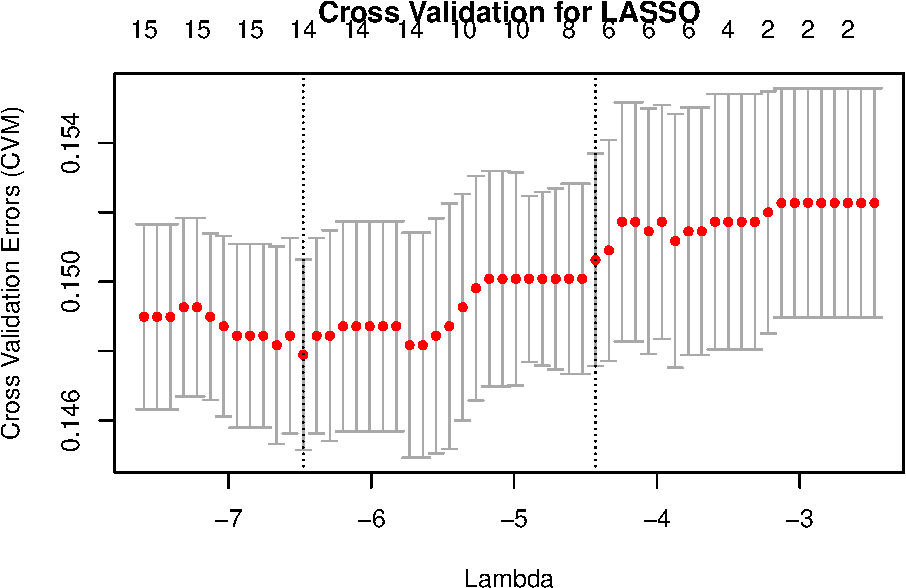
\includegraphics{HW3_Wu-Yulun_files/figure-latex/unnamed-chunk-22-1.pdf}
The curve is not a typical U-curve. I don't think we need regularization
here, because CVM doesn't change much with different \(\lambda\).

\end{document}
